\chapter{Introducción a los sistemas de comunicación}

\section{Introducción}

Desde el principio de los tiempos, el ser humano se ha comunicado con sus congéneres de distintas maneras: comenzó a través de la voz (se cree que hace unos 100.000 años), con algún tipo de protolenguaje, para posteriormente comenzar a utilizar sistemas de comunicaciones permanentes (la escritura).

Por todos es conocido la evolución histórica de distintos sistemas escritos, entre los que podemos destacar (\href{https://es.wikipedia.org/wiki/Anexo:Cronolog%C3%ADa_de_las_tecnolog%C3%ADas_de_la_comunicaci%C3%B3n}{referencia}):
\begin{itemize}
    \item \textbf{Pinturas rupestres}: Realizadas en cuevas o rocas en las que se pueden observar escenas de caza, distintos animales, grabado de manos, figuras humanas... Algunas de las pinturas encontradas cuentan con más de 50.000 años. Tenemos un ejemplo cercano en las \href{https://es.wikipedia.org/wiki/Cueva_de_Santimami\%C3\%B1e}{cuevas de Santimamiñe} en donde tenemos pinturas datadas entre 14.000 y 9.000 años a. C.

    \item \textbf{Escritura cuneiforme}: Es uno de los primeros sistemas de escritura realizados, y se utilizaban tablillas de arcilla húmeda en las que se grababa mediante un tallo vegetal. Con este sistema se han datado tablas anteriores al 3.200 a.C. y en distintos idiomas.

    \item \textbf{Escritura jeroglífica y el papiro}: En el antiguo Egipto se crea la escritura mediante signos que comienza por escribirse en paredes para posteriormente inventar el papiro (cuya datación más antigua es del 2.500 a.C.) y de esta manera se comienza a tener un sistema de comunicación fácilmente manejable e intercambiable.

    \item \textbf{Uso de palomas mensajeras}: El uso de palomas mensajeras para el envío de comunicaciones data de la época anterior a 1.500 a.C. y se ha estado utilizando hasta este siglo en algunos países durante desastres naturales.

    \item \textbf{Telégrafo}: A partir de mediados del siglo XVIII y durante el inicio del siglo XIX hubo bastantes avances en las investigaciones del electromagnetismo y de esta manera se comenzó a investigar cómo usarlo para el envío de señales. En 1837 Samuel Morse patenta el \href{https://es.wikipedia.org/wiki/Tel%C3%A9grafo#Historia_del_tel%C3%A9grafo}{telégrafo}. En \textbf{1858} se une Irlanda y Terranova mediante el \textbf{primer cable trasatlántico}.

    \item \textbf{Teléfono}: Como evolución al telégrafo, que sólo permitía el envío de señales, nace el teléfono de la mano de \href{https://es.wikipedia.org/wiki/Antonio_Meucci}{Antonio Meucci} (aunque normalmente se le atribuye el invento a \href{https://es.wikipedia.org/wiki/Alexander_Graham_Bell}{Alexander Graham Bell}). En 1860 realizó una demostración pública transmitiendo voz a una considerable distancia.
\end{itemize}

Tal como podemos ver, ha habido distintos sistemas de comunicación utilizados durante siglos para el envío y recepción de información.

\section{Comunicación de la información}

Tal como hemos visto, los sistemas de comunicación de la información no es algo nuevo, ¿pero qué necesidades tiene un sistema de comunicación?

\begin{itemize}
    \item \textbf{Emisor}: Es el origen y la fuente de la información que se pretende comunicar.
    \item \textbf{Receptor}: Es el destinatario, el que va a recibir la información.
    \item \textbf{Mensaje}: Es la información que queremos transmitir entre el emisor y el recepetor.
    \item \textbf{Código}: Es el conjunto de reglas utilizadas a la hora de representar el mensaje. El emisor y receptor deben utilizar el mismo código para que la comnunicación sea correcta.
    \item \textbf{Canal}: Es el medio físico por el que se va a enviar el mensaje.
    \item \textbf{Señal}: Es el componente físico por el que se envía la información.
\end{itemize}

Para entender de mejor manera un sistema de comunicación y los componentes que lo forman, vamos a poner dos ejemplos:

\subsubsection*{Ejemplo 1: Comunicación oral}

\begin{wrapfigure}{r}{0.25\linewidth}
    \centering
    \vspace{-35pt}
    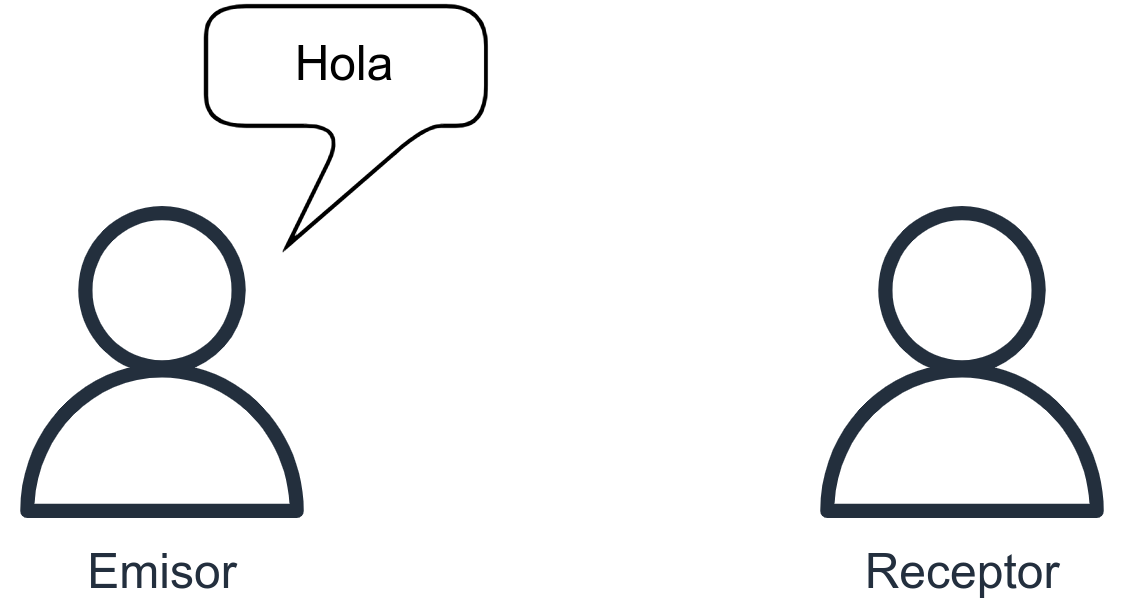
\includegraphics[width=\linewidth]{comunicacion-1.png}
    \vspace{-30pt}
\end{wrapfigure}
En este ejemplo vemos que hay dos personas, las cuales se han identificado cada una de ellas como “Emisor” y “Receptor”, y así de esta manera conocemos quién es el origen y quién el destino de la comunicación.

En este caso, el \textbf{mensaje} es “Hola”, haciendo uso del \textbf{código} conocido como “castellano”. La \textbf{señal} que se va a utilizar es la voz, ya que están hablando y el \textbf{canal} por el que se envía el mensaje es el aire.

Es un ejemplo sencillo que utilizamos cada día.

\subsubsection*{Ejemplo 2: Comunicación escrita por mensajería}

\begin{wrapfigure}{r}{0.25\linewidth}
    \centering
    \vspace{-35pt}
    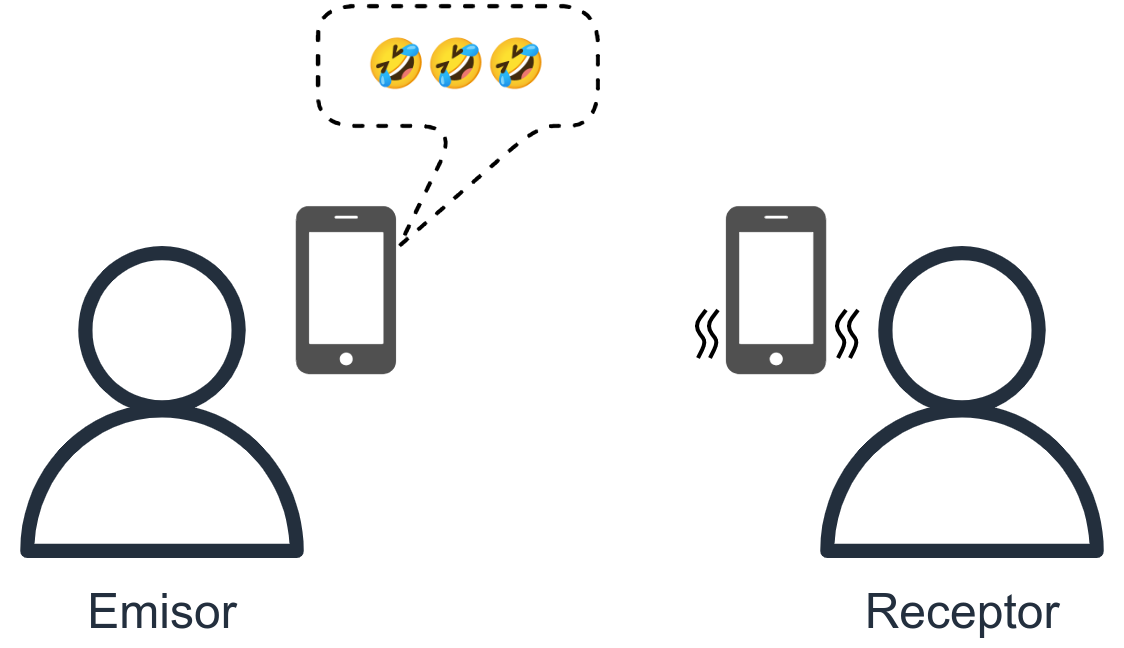
\includegraphics[width=\linewidth]{comunicacion-2.png}
    \vspace{-30pt}
\end{wrapfigure}
AL igual que en el ejemplo anterior, vemos que hay dos personas, las cuales se han identificado cada una de ellas como “Emisor” y “Receptor” pero que en este caso se van a comunicar haciendo uso de un teléfono móvil, tal como hacemos en nuestro día a día a través de una aplicación de mensajería o red social.

Teniendo en cuenta esto, en este ejemplo realmente existen dos sistemas de comunicación que están mezclados y uno está por encima del otro:

\begin{itemize}
    \item \textbf{Entre personas}: Similar al ejemplo anterior, el emisor y el receptor se están comunicando, con el mensaje compuesto por tres \href{https://es.wikipedia.org/wiki/Emoji}{emojis} que representan estar riendo. El \textbf{código} es el idioma que estén utilizando, el \textbf{canal} sería el programa utilizado y la \textbf{señal} podríamos decir que es el móvil.

    \item \textbf{Entre dispositivos}: En este caso, el emisor y receptor es el móvil de cada usuario. El mensaje es el mismo, pero convertido a un sistema digital (como el \hyperlink{binario}{binario}). El \textbf{canal} en este caso sería el aire y la \textbf{señal} es la utilizada por el móvil, por ejemplo el 5G.
\end{itemize}

Tal como se puede ver en este caso, una comunicación puede depender a su vez de otro sistema de comunicación.

\subsection{Esquema de la comunicación}
Para simplificar cómo se realiza la comunicación, podemos utilizar el siguiente esquema:

\begin{center}
    \vspace{-10pt}
    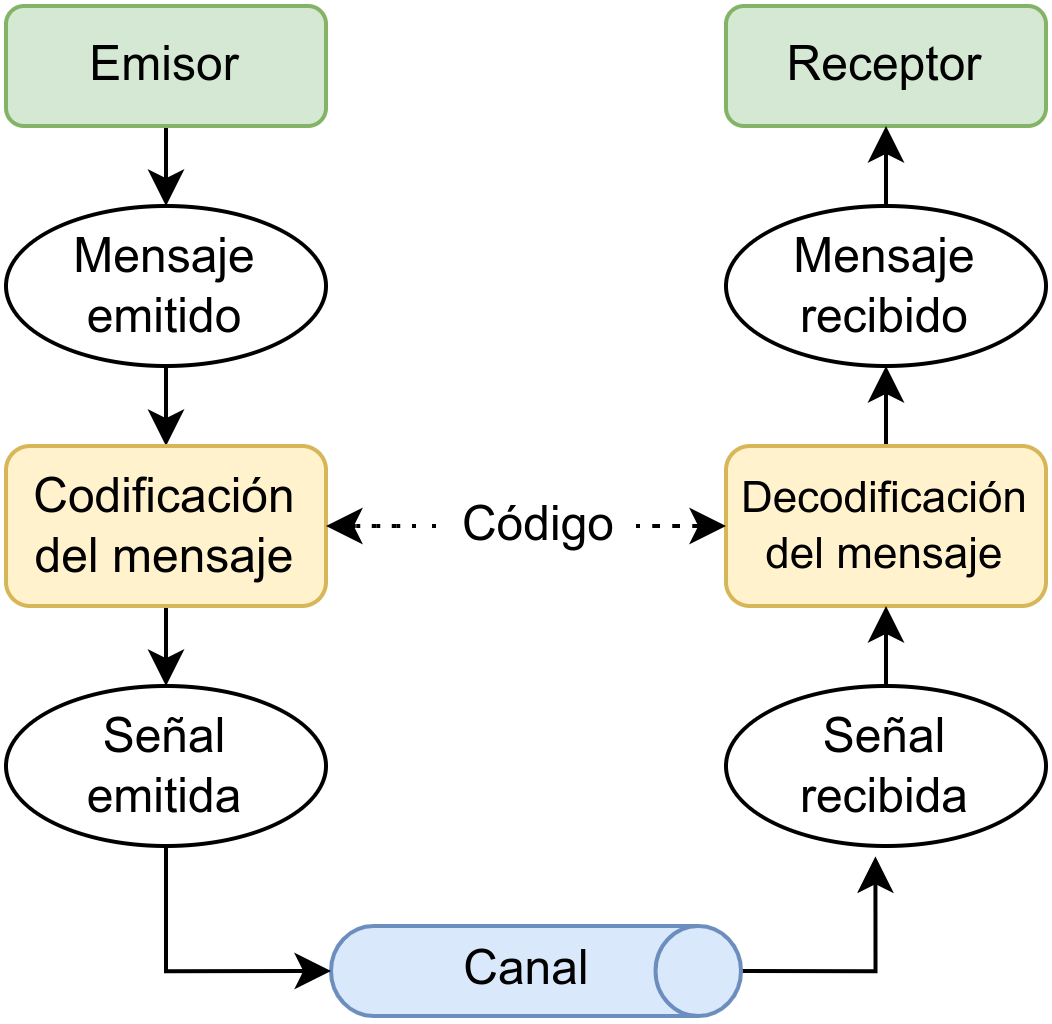
\includegraphics[width=0.6\linewidth]{comunicacion-esquema.png}
    \vspace{-10pt}
\end{center}


\section{Sistemas de numeración}
La información que queremos retransmitir debe estar representada de alguna manera, y tal como hemos visto previamente, \textbf{a través de un código que tanto emisor como receptor deben conocer}.

En sistemas orales, o escritos, lo habitual es hacer uso de un idioma concreto mediante un alfabeto conocido. En informática se hace uso de distintos sistemas de numeración para representar tanto números como el resto de información.

\subsection{Sistema decimal}
El ser humano, desde hace tiempo ha utilizado como sistema para contar el sistema decimal, representado mediante el sistema \href{https://es.wikipedia.org/wiki/N%C3%BAmeros_ar%C3%A1bigos}{arábigo}. Posiblemente se adoptó este sistema por contar con 10 dedos en las manos.

El sistema numérico decimal está basado en diez símbolos ordenados (0, 1, 2, 3, 4, 5, 6, 7, 8, 9), situados de manera ponderada (cada posición tiene un peso específico), que permiten representar las cantidades deseadas. Debido a que hacemos uso de diez símbolos se dice que utiliza la \textbf{base 10}.

\subsubsection*{Representación}
Cuando se combina con otros sistemas de numeración, debemos indicar la base en la forma $ \mathbf{19_{(10}} $ , es decir, poniendo un pequeño “\textbf{(10}” a la derecha del número representado la base 10.

La representación de cualquier combinación del sistema decimal se puede representar en forma de potencia, donde la base es 10 (como ya hemos visto antes) y el exponente es la posición en la que se sitúa el símbolo.

Vamos a tomar como ejemplo el siguiente número: \textbf{146}. La representación en forma de potencias:

\begin{center}
    \vspace{-10pt}
    $ 146 =1\times10^2 + 4\times10^1 + 6\times10^0 $

    $ 146 = 1\times100 + 4\times10 + 6\times1 $

    $ 146 = 100+40+6 $
\end{center}

Como se puede comprobar, lo que hemos hecho ha sido coger cada símbolo representado y lo hemos multiplicado por la base (en este caso base 10) y a la base le hemos puesto el exponente de la posición en la que se encuentra. \textbf{El símbolo de más a la derecha tiene como exponente el cero}, y hacia la izquierda el exponente se incrementa en uno para cada posición.


\hypertarget{binario}{}
\subsection{Sistema binario}

En informática el sistema binario es el más importante ya que es el sistema que internamente utilizan los circuitos digitales. En este sistema sólo se hace uso de dos símbolos, el “0” y el “1”, y por tanto \textbf{su base es 2}. Los dos dígitos se denominan \textbf{bits} (contracción de \textbf{binary digit}).

\subsubsection*{Representación}

Para representar que estamos haciendo uso del sistema binario debemos indicar la base al lado del número, por ejemplo: $\mathbf{ 101001_{(2}} $. Como se puede ver es añadir “\textbf{(2}” en pequeño al final del último símbolo.


\subsection{Sistema hexadecimal}

Esta vez necesitamos dieciséis símbolos ordenados, así que es un sistema de \textbf{base 16}. Para la representación se hace uso de los símbolos numéricos que conocemos (0, 1, 2, 3, 4, 5, 6, 7, 8, 9) y para representar los siguientes, las letras “A”, “B”, “C”, “D”, “E” y “F”, de esta manera formamos los 16 símbolos que necesitamos.

Teniendo en cuenta esto, podemos hacer la representación directa de que $\mathbf{A_{(16} = 10_{(10}}$ y que $\mathbf{E_{(16} = 14_{(10}}$.

En informática es muy habitual hacer uso del sistema hexadecimal a la hora de trabajar con \textbf{bytes} (que es una “palabra” de \textbf{8 bits}). Un símbolo hexadecimal se representa como 4 bits, por lo que necesitaríamos 2 símbolos hexadecimales para un byte.

También se usa durante la edición de código en formato de datos, o durante la programación en ensamblador.

\subsubsection*{Representación}
Al igual que con los sistemas anteriores, debemos añadir la base cuando estemos utilizando el sistema hexadecimal: $\mathbf{ F17A_{(16}} $ , $\mathbf{ FBE1D_{(16}} $ , $\mathbf{ 1FAB27_{(16}} $


\subsection{Sistema octal}
En ordenadores antiguos era habitual hacer uso del sistema octal. Hoy día se usa más como sistema intermedio entre binario y hexadecimal.

Esta vez nos basamos en ocho símbolos ordenados (0, 1, 2, 3, 4, 5, 6, 7), que, al combinarlos, permiten representar las cantidades deseadas. Debido a que hacemos uso de ocho símbolos se dice que utiliza la \textbf{base 8}.

\subsubsection*{Representación}
Para representar la base, debemos añadir “(8” a la derecha del número que hayamos indicado, como por ejemplo: $\mathbf{ 770_{(8} }$ , $\mathbf{ 175_{(8}} $


\subsection{Conversiones entre los distintos sistemas de numeración}

Hasta ahora no nos habíamos encontrado con distintos sistemas de numeración, pero ahora que conocemos cuatro de ellos, tenemos que saber que existe la posibilidad de realizar conversiones entre ellos.


Una vez entendidos los distintos sistemas de numeración nos tiene que quedar claro que aunque la representación de los símbolos sea la misma, el número o cantidad representada no es la misma. Por ejemplo:

\errorbox{
    \begin{center}
        $\mathbf{ 1010_{(10}  \neq  1010_{(2}  \neq  1010_{(16}  \neq 1010_{(8}} $
    \end{center}
}

A continuación se va a explicar cómo realizar conversiones entre los distintos sistemas de numeración que hemos visto, y a modo de resumen está la \hyperlink{tabla_conversiones_directas}{tabla de conversiones directa}.

\subsubsection{Conversión de decimal a...}
La manera más sencilla para realizar las distintas conversiones partiendo de un número decimal es hacer divisiones sucesivas usando la base a la que queremos realizar la conversión.

\subsubsection*{... binario}
Se trata de dividir sucesivamente el número decimal y los sucesivos cocientes entre dos (la base binaria).

Vamos a utilizar como ejemplo el número decimal $\mathbf{27_{(10}}$ :

\begin{center}
    \vspace{-20pt}
    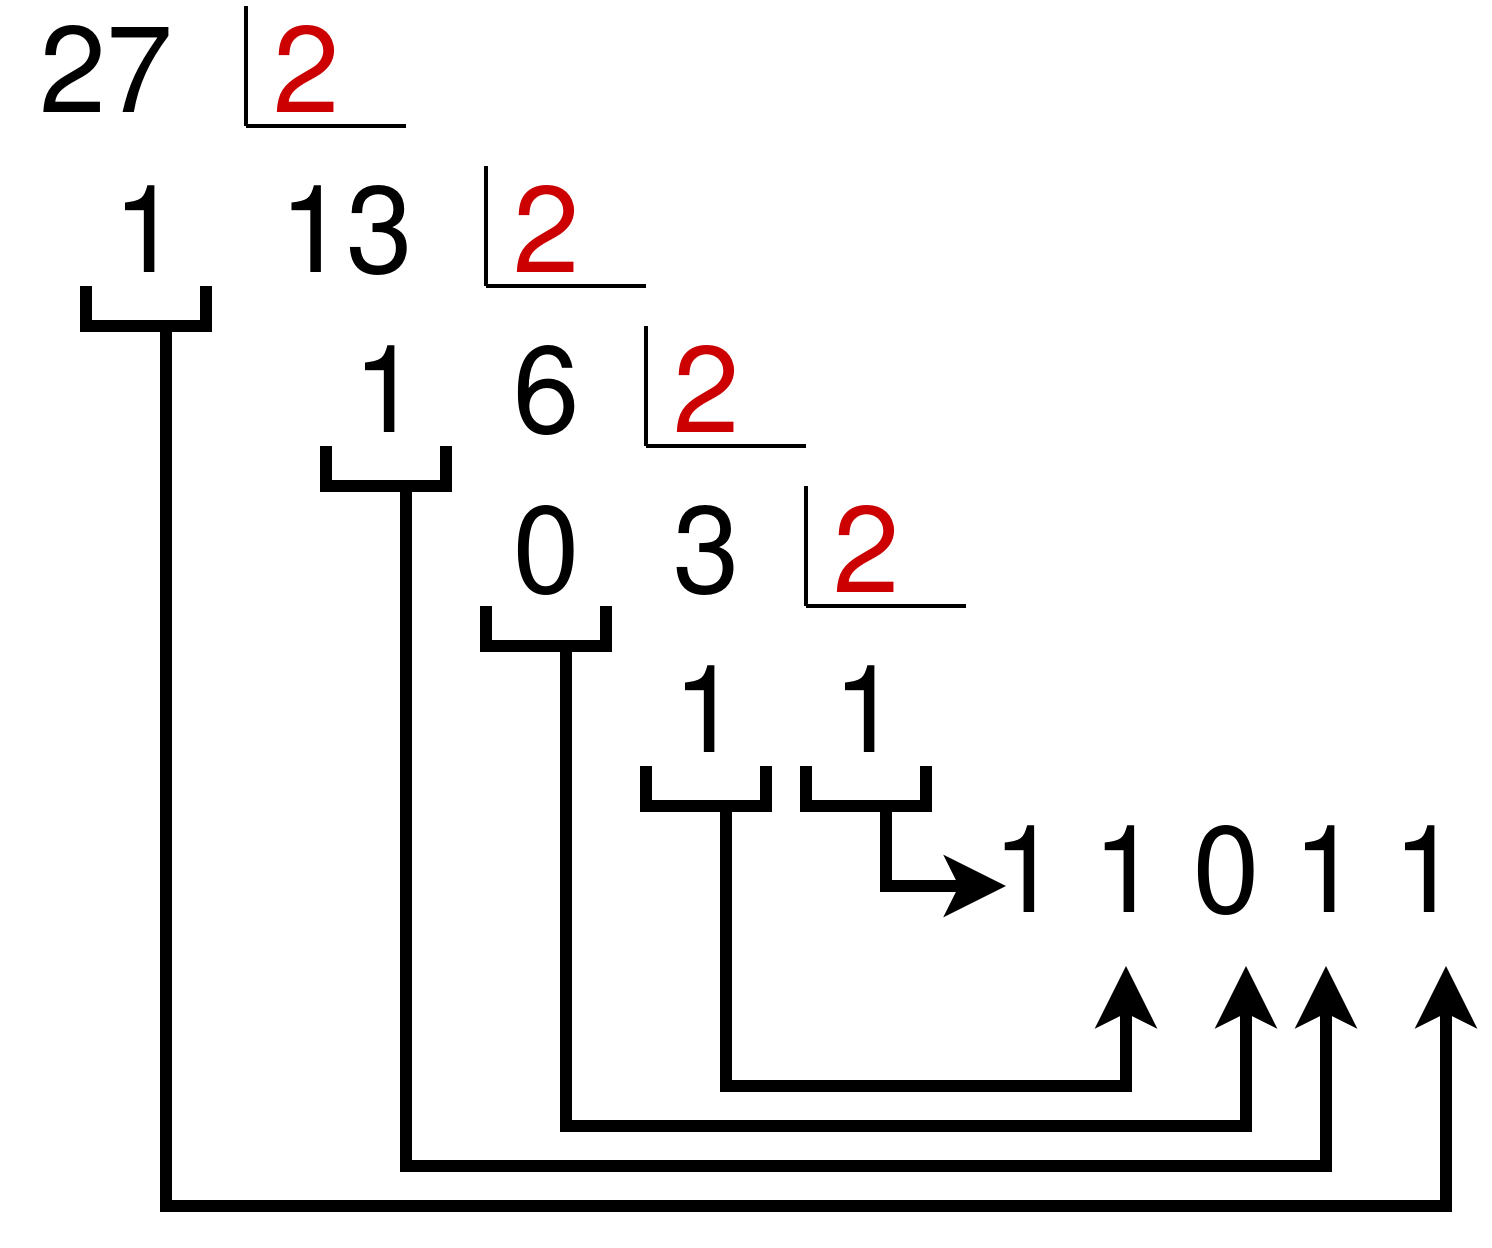
\includegraphics[width=0.29\linewidth]{decimal_binario.png}
    \vspace{-20pt}
\end{center}

\textbf{Los restos los cogemos en orden inverso} para obtener la siguiente equivalencia: $\mathbf{27_{(10} = 11011_{(2}}$

\subsubsection*{... hexadecimal}
Se trata de dividir sucesivamente el número decimal y los sucesivos cocientes entre 16 (la base hexadecimal). Cuando el cociente o resto sea entre 10 y 15, habrá que cambiarlo por la letra correspondiente.

\begin{center}
    \vspace{-10pt}
    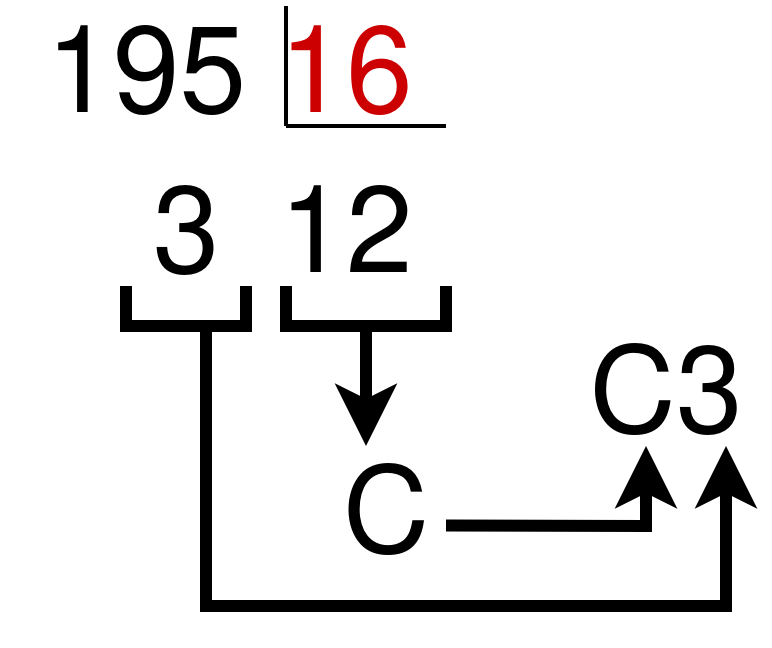
\includegraphics[width=0.2\linewidth]{decimal_hexadecimal.png}
    \vspace{-15pt}
\end{center}

\textbf{Los restos los cogemos en orden inverso} para obtener la siguiente equivalencia: $\mathbf{195_{(10} = C3_{(16}}$

\subsubsection*{... octal}
Al igual que los anteriores, hacemos divisiones sucesivas:

\begin{center}
    \vspace{-10pt}
    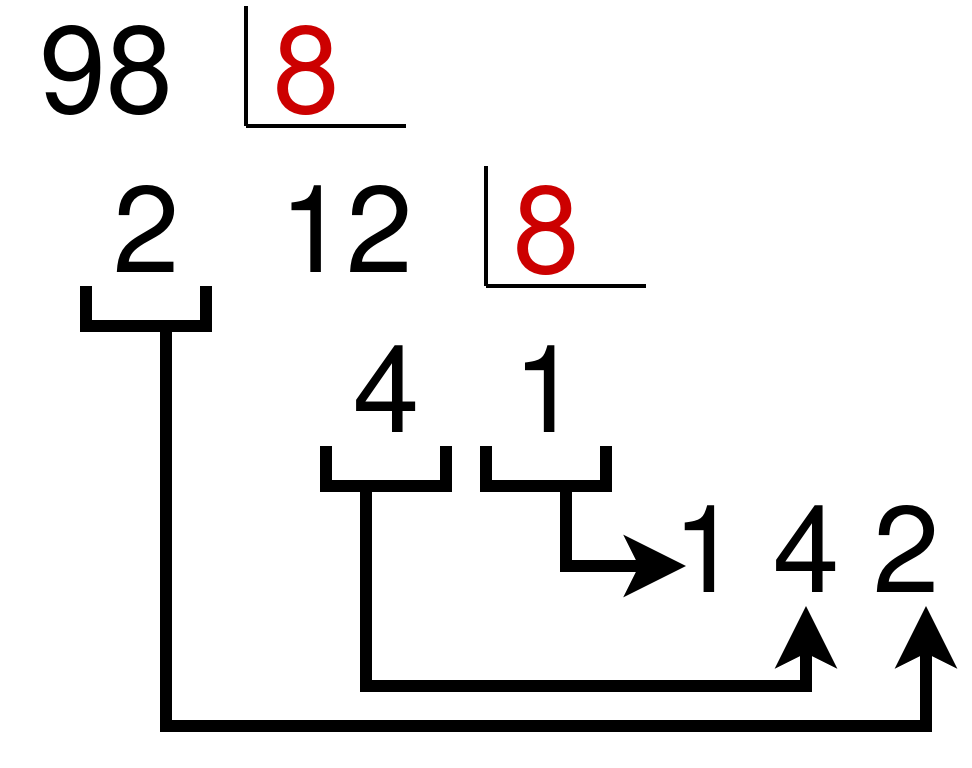
\includegraphics[width=0.25\linewidth]{decimal_octal.png}
    \vspace{-15pt}
\end{center}

\textbf{Los restos los cogemos en orden inverso} para obtener la siguiente equivalencia: $\mathbf{98_{(10} = 142_{(8}}$


\subsubsection{Conversión de binario a...}

\subsubsection*{... decimal}
El sistema de numeración binario es un sistema posicional donde cada dígito binario (bit) tiene un valor basado en su posición relativa al \textbf{LSB} (\textit{Least Significant Bit} = bit menos significativo, que es el que está más a la derecha y que tiene el menor valor).

Cualquier número binario puede convertirse a su equivalente decimal multiplicando cada bit por la base (2) y usando como exponente la posición (siendo 0 el exponente del bit de más a la derecha). Para ilustrarlo, cojamos como ejemplo el número binario $\mathbf{11011_{(2}}$:

\begin{center}
    \vspace{-20pt}

    $ \mathbf{11011_{(2}} $

    $ \mathbf{1\times2^4 + 1\times2^3 + 0\times2^2 + 1\times2^1 + 1\times2^0} $

    $ \mathbf{16 + 8 + 0 + 2 + 1 = 27_{(10}} $
    \vspace{-15pt}
\end{center}

Nótese que el procedimiento consiste en determinar los valores (es decir, las potencias de 2) de cada posición de bit que contenga un 1 y luego sumarlos.

Nótese también que el \textbf{MSB} (\textit{Most Significant Bit} = bit más significativo, el que está más a la izquierda, el que tiene mayor valor) tiene un valor de $\mathbf{2^4}$ a pesar de que es el quinto bit. Esto se debe a que el \textbf{LSB} (\textit{Least Significant Bit}, el bit menos significativo, el que está a la derecha) es el primer bit y tiene un valor de $\mathbf{2^0}$.

\subsubsection*{... octal}
Para convertir un número binario a octal \textbf{se agrupan los dígitos de 3 en 3 empezando desde el lado derecho} hacia la izquierda, sustituyendo cada trío de dígitos binarios por su equivalente en octal.

Si en el lado izquierdo quedase algún bit “suelto” (sin formar un grupo de 3), se pueden poner “0” a la izquierda.

Cogemos como ejemplo el número binario $\mathbf{1100101001001_{(2}}$ para pasarlo a octal, haremos:

\begin{center}
    \vspace{-15pt}
    $\mathbf{001\ \ 100\ \ 101\ \ 001\ \ 001_{(2} = 14511_{(8}}$
    \vspace{-15pt}
\end{center}

\subsubsection*{... hexadecimal}
Similar al caso anterior, pero en este caso \textbf{la agrupación que se realiza debe de ser de 4 en 4 bits}. Si usamos el mismo ejemplo anterior $\mathbf{1100101001001_{(2}}$ :

\begin{center}
    \vspace{-15pt}
    $\mathbf{0001\ \ 1001\ \ 0100\ \ 1001_{(2} = 1949_{(16}}$
    \vspace{25pt}
\end{center}



\subsubsection{Conversión de hexadecimal a...}
\subsubsection*{... binario}
Para pasar de hexadecimal a binario convertiremos cada símbolo hexadecimal a 4 dígitos binarios.

\begin{center}
    \vspace{-15pt}
    $\mathbf{F17A_{(16} = 1111\ \ 0001\ \ 0111\ \ 1010_{(2}}$

    $\mathbf{1A4F_{(16} = 0001\ \ 1010\ \ 0100\ \ 111_{(2}}$
    \vspace{-15pt}
\end{center}


\subsubsection*{... decimal}
Al igual que hemos hecho con las conversiones previas a decimal, se podría realizar haciendo potencias de 16, pero se entiende que es más complicado de realizar.

Por lo tanto, \textbf{la manera más sencilla es pasar primero a binario} como acabamos de ver \textbf{y posteriormente convertir ese binario a decimal} como hemos visto previamente.

\subsubsection*{... octal}
Pasar primero a binario y después a octal.



\subsubsection{Conversión de octal a...}
\subsubsection*{... binario}
Cada dígito en octal se convierte en su representación en 3 bits:

\begin{center}
    \vspace{-15pt}
    $\mathbf{167_{(8} = 001\ \ 110\ \ 111_{(2}}$

    $\mathbf{253_{(8} = 010\ \ 101\ \ 011_{(2}}$
    \vspace{-15pt}
\end{center}
Los ceros de la izquierda se podrían quitar, ya que no alteran el valor.

\subsubsection*{... decimal}
Se puede realizar de dos maneras. La primera es hacer uso de potencias de 8 (similar al paso de pasar de binario a decimal, pero cambiando la base):

\begin{center}
    \vspace{-15pt}
    $\mathbf{157_{(8} = 1\times8^2 + 5\times8^1 + 7\times8^0 = }$

    $\mathbf{1\times64 + 5\times8 + 7\times1 = }$

    $\mathbf{64 + 40 + 7 = 111_{(10}}$

    Resultado: $\mathbf{157_{(8} = 111_{(10}}$
    \vspace{-15pt}
\end{center}

Con números grandes puede ser un poco complicado calcular las potencias de 8, por lo que \textbf{la alternativa es pasarlo primero a binario} como hemos visto, \textbf{y después pasarlo de binario a decimal}.

\subsubsection*{... hexadecimal}
La manera más sencilla es realizar la conversión primero a binario tal como hemos visto, y posteriormente pasar el número binario a hexadecimal como se ha visto previamente.


\chapter{Redes de comunicación}
En el ámbito informático una red de comunicaciones es representada como una red de ordenadores. Las redes de ordenadores son un conjunto de equipos hardware que están conectados entre sí (ya sea mediante cables o de manera inalámbrica) y que a través de un software especializado envían y reciben impulsos eléctricos (u ondas electromagnética) para el transporte de datos. De esta manera podrán compartir información, recursos u ofrecer servicios.


\section{Breve historia de las redes}
A continuación una breve cronología mostrando los hitos más importantes dentro de las redes de comunicaciones, en lo que a ordenadores se refiere (\href{https://en.wikipedia.org/wiki/Computer_network}{Referencia}).

\begin{description}
    \item[\textasciitilde 1950]
    En la década de los 50 se desarrollan los circuitos integrados. Esto hará que en el futuro los ordenadores cada vez se vayan haciendo más pequeños.

    Las redes de ordenadores comienzan a aparecer en las bases militares americanas, en principio para sistemas de radares.

    \item[\char`\~ 1960]
    Se realiza una conexión entre dos mainframes en EEUU para el sistema de reservas aéreas comerciales.

    El \href{https://es.wikipedia.org/wiki/Instituto_de_Tecnolog%C3%ADa_de_Massachusetts}{MIT} utiliza un ordenador para enrutar y mantener conexiones telefónicas.

    En 1966, aparece un paper (artículo científico) describiendo las WAN.

    En 1969 ARPANET (red de ordenadores creadas por el Departamento de Defensa de Estados Unidos) cuenta con 4 nodos (a 50kbit/s de velocidad).

    \item[\char`\~ 1970]
    En 1972 se hace la primera demostración pública de ARPANET.

    A comienzos de la década (1973) se crea Ethernet en la compañía Xerox Parc.

    A finales de la década Xerox intenta hacer que Ethernet se convierta en un estándar de conexión para terminar con las competencias (token ring, …).

    \begin{center}
        \vspace{-10pt}
        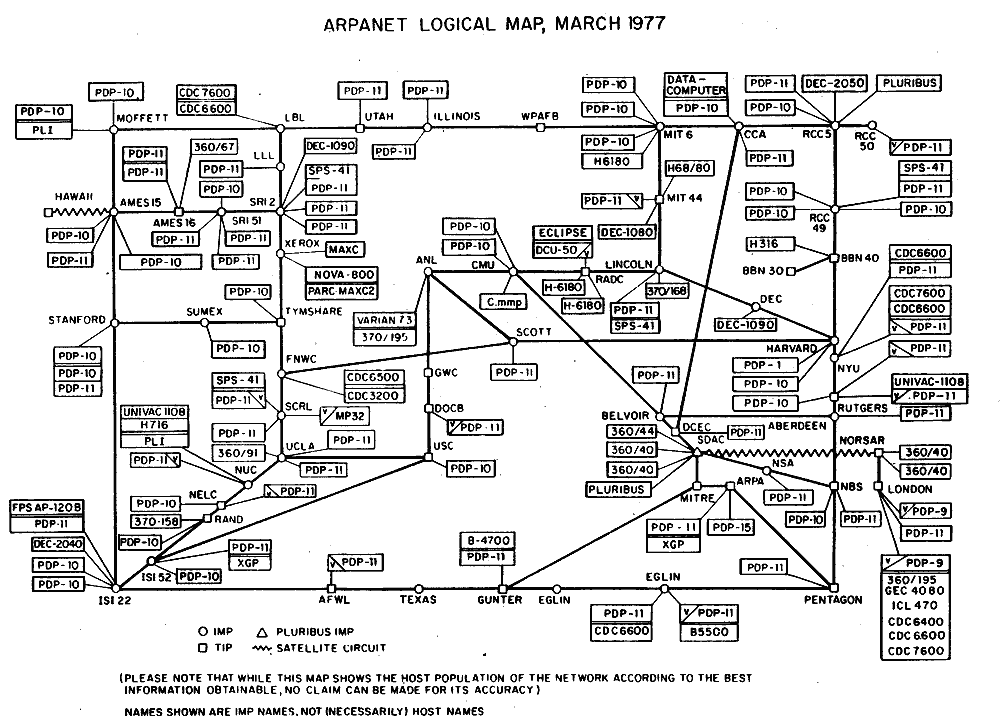
\includegraphics[frame,width=0.9\linewidth]{Arpanet_logical_map_march_1977.png}
        \vspace{-5pt}
        \captionof{figure}{Mapa lógico de ARPANET, marzo de 1977. Origen: \href{https://es.wikipedia.org/wiki/ARPANET\#/media/Archivo:Arpanet_logical_map,_march_1977.png}{ Wikipedia}}\vspace{-13pt}
    \end{center}

    \item[\char`\~ 1980]
    Los ordenadores personales empiezan a generalizarse.

    Aparece el protocolo para enviar y recibir e-mails (SMTP).

    El protocolo TCP/IP se convierte en el utilizado por ARPANET (1983) y es declarado como su estándar para las comunicaciones.

    Aparece el servicio DNS.

    Se crea el modelo de referencia OSI.

    Aparece el primer gusano por la red (Morris worm, 1988). Se estima que infectó al 10\% de los ordenadores conectados a la red.

    Se crea el protocolo BGP.

    El protocolo Ethernet evoluciona y permite conexiones a 10Mbit/s.


    \item[\char`\~ 1990]
    Tim Berners-Lee desarrolla el código para WWW y crea el primer servidor web (1991).

    Se puede decir que aquí es cuando nace la Internet que conocemos actualmente.

    En 1995 Ethernet permite conexiones a 100Mbit/s

    Se establece un control para los nombres de dominio (posteriormente lo asumirá ICANN).

    Aparece Amazon, ebay, Craiglist, IMDB, hotmail, google, yahoo, ...

    Aparece el protocolo IPv6 (1998).

    Aparece el protocolo wifi 802.11b.

    \item[\char`\~ 2000]
    Crisis de las “.com”.

    Internet se generaliza.

    Empiezan a permitirse más TLDs, que no corresponden sólo a países.

    Ethernet permite conexiones a 1Gbit/s

    \item[\char`\~ 2010]
    Ethernet permite conexiones a 400Gbit/s (2018).

    \href{https://en.wikipedia.org/wiki/Starlink}{Starlink} comienza a desplegar su constelación de satélites para dar cobertura en todo el planeta.


\end{description}

\section{Tipos de redes}
A la hora de diferenciar las redes de ordenadores podemos diferenciarlas por distintos conceptos:

\begin{itemize}
    \item Por el medio de transmisión utilizado.
    \item Por la dirección de los datos.
    \item Por el alcance.
    \item Por el grado de acceso.
    \item Por la topología.
    \item ...
\end{itemize}

\subsection{Por el medio de transmisión utilizado}
Más adelante veremos distintos \hyperlink{sistemas_transmision}{sistemas de transmisión}, pero para ir diferenciando podemos crear dos grandes grupos teniendo en cuenta el medio utilizado:

\begin{itemize}
    \item \textbf{Guiados}: Es decir, a través de cables que se encargarn de realizar la transmisión de la señal desde un punto de origen al punto de destino.

    \item \textbf{No guiados}: Se hace uso de algún sistema inalámbrico (mediante antenas) para realizar la transmisión de los datos.
\end{itemize}


\subsection{Por la dirección de los datos}
Si tenemos en cuenta la dirección de los datos en la transmisión, podemos diferenciarlos como:

\begin{itemize}
    \item \textbf{Simplex}: la comunicación sólo se realiza en un único sentido, por lo que sólo es necesario un único canal de transmisión.

    \item \textbf{Half-duplex}: se permite la comunicación en ambos sentidos, pero no de manera simultánea, por lo que emisor y receptor se reparten el tiempo de emisión. Por ejemplo, el \textit{\textbf{walkie-talkie}}.

    \item \textbf{Duplex}: O también conocido como \textit{full-duplex}, permite la comunicación en ambas direcciones y de manera simultánea. Por ejemplo, el \textbf{teléfono}. Para ello es necesario tener una de estas dos opciones:
    \begin{itemize}
        \item Dos canales Half-duplex: uno para cada dirección de la comunicación.
        \item Un único canal por el que se envía la comunicación, pero para ello es necesario algún sistema de multiplexación (como puede ser usar frecuencias separadas).
    \end{itemize}
\end{itemize}


\subsection{Por alcance}
Teniendo en cuenta el alcance al que llegan las redes, podríamos realizar la siguiente distinción:

\subsubsection{Red de área personal (PAN)}
Del inglés \textit{Personal Area Network}, es aquella en la que interactúan distintos dispositivos de muy corto alcance, limitado al área de una persona.

El ejemplo más habitual hoy día sería la comunicación mediante tecnología inalámbrica por Bluetooth en la comunicación entre ordenador, móvil y dispositivos como un \textit{smartwatch}.


\subsubsection{Red de área local (LAN)}
Del inglés \textit{Local Area Network}, es una red que puede abarcar un cierto área de tamaño como una casa, una oficina, un colegio, una universidad...

El ejemplo de una oficina sería una red en la que existen distintos ordenadores, que pueden comunicarse entre sí o compartir información con un servidor ya sea a través de una red cableada o también inalámbrica.

\subsubsection{Red de área metropolitana (MAN)}
Del inglés \textit{Metropolitan Area Network}, y como su nombre indica, el área es mayor y suele abarcar una ciudad para ofrecer los servicios necesarios en la misma.

En este caso también puede ser de manera cableada (normalmente haciendo uso de tecnología más rápida como es la fibra óptica) y también de manera inalámbrica.

Dentro de los servicios que pertenecerían a una MAN podemos poner como ejemplos:
\begin{itemize}
    \item Despliegue de zonas WIFI gratuito en la ciudad.
    \item Comunicación entre sistemas de información (paradas de autobuses, marquesinas, ...).
    \item Sistemas de video-vigilancia municipal.
\end{itemize}

Algunos de estos servicios que están en una MAN pueden ser públicos (como el WIFI) o de acceso restringido (sistemas de seguridad).

\subsubsection{Red de área amplia (WAN)}
Del inglés \textit{Wide Area Network}, es una red que abarca grandes extensiones geográficas y normalmente construidas por grandes empresas o proveedores de internet (ISP, \textit{Internet Service Provider}).


\subsection{Por el grado de acceso}
Teniendo en cuenta quién puede acceder a la red, podríamos definir dos tipos de redes:

\begin{itemize}
    \item \textbf{Red privada}: es una red que sólo ciertas personas pueden acceder y que no normalmente no es accesible desde otras redes. El ejemplo más sencillo es la red que tenemos en casa.
    \item \textbf{Red pública}: es una red a la que puede acceder cualquier persona y que interconecta otras redes sin importar su situación geográfica. Internet es una red pública.
\end{itemize}

\subsection{Por la topología}
La topología de una red indica cómo están interconectados los nodos de la misma y el camino que pueden realizar los datos cuando viajan por esa red. En resumen: \textbf{es el diseño de la red}.

%TODO: completar información






\chapter{Arquitectura en capas}
Un sistema de comunicación se pueden diferenciar en distintos niveles en los que cada uno realiza una función independiente, pero que a su vez interactúan con los niveles limítrofes.

\begin{center}
    \vspace{-10pt}
    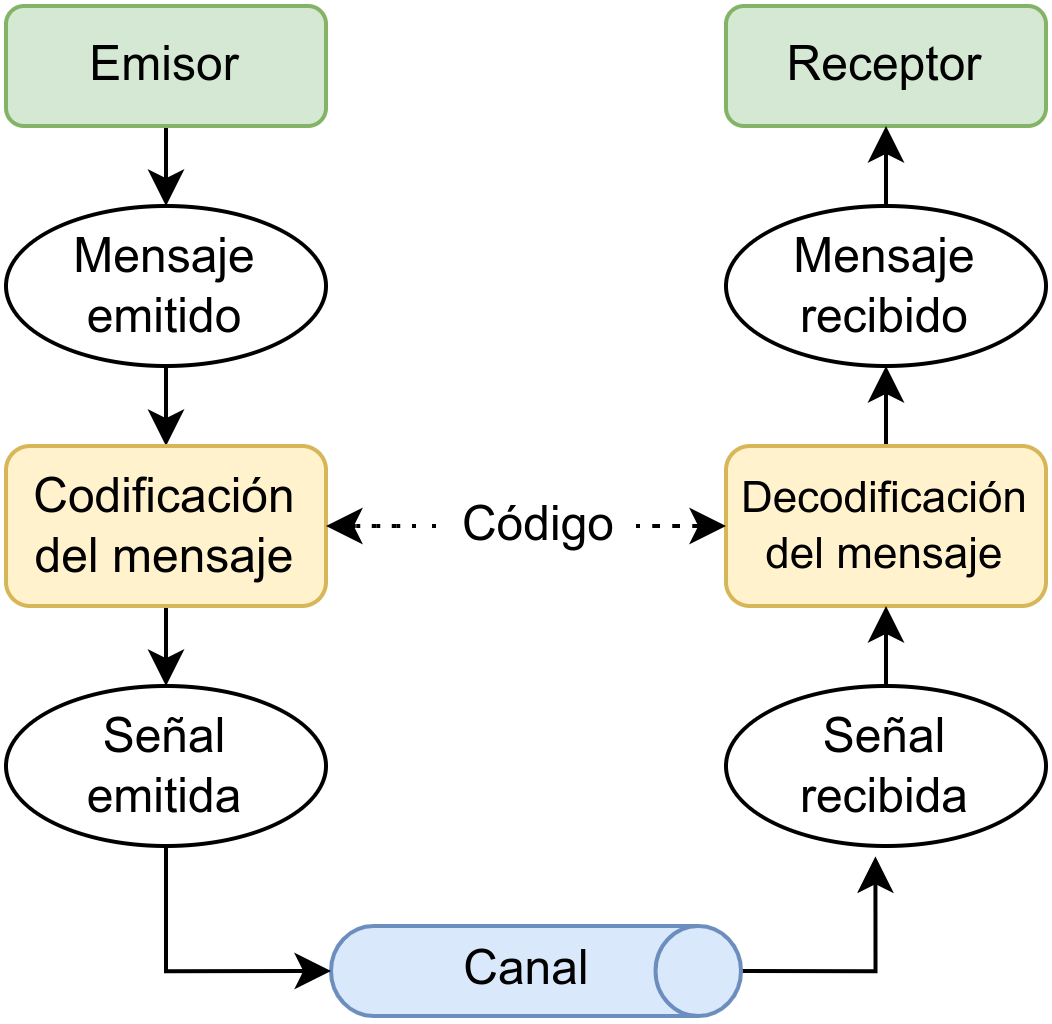
\includegraphics[width=0.4\linewidth]{comunicacion-esquema.png}
    \vspace{-10pt}
\end{center}

Este ejemplo es un modelo simplificado de comunicación, y dentro de una arquitectura de red de ordenadores pueden existir más capas en las que pueden existir distintas funciones extra que no aparecen en este esquema.

\section{Origen}

Al comienzo de las redes de ordenadores cada empresa creaba su propio sistema de comunicación creando su propio hardware y software, lo que hacía imposible la interconexión entre equipamiento de distintas empresas.

Estos sistemas de comunicación constan de unas reglas que los nodos deben conocer para poder comunicarse entre sí, y a ese conjunto de reglas se les denomina \textbf{protocolo de comunicación}.


Para que eso hoy en día no suceda ya que las redes están definidas en varios estándares, como veremos más adelante.

\infobox{Un \textbf{estándar} es un conjunto de normas que pueden abarcar distintos niveles (tanto software como hardware) que ha sido aceptado, o creado, por la gran mayoría de las empresas del sector para poder realizar la interconexión e intercomunicación entre sí.}


\section{Ventajas de la división en capas}

La división en capas nos permite:
\begin{itemize}
    \item Dividir el proceso de comunicación en procesos más pequeños.

    \item Aislar las funciones de cada capa. De esta manera, en caso de realizar modificaciones en la misma, no afecta al resto de capas.

    \item Ocultar la implementación al resto de capas. Siguiendo con el punto anterior, una capa utilizará los servicios de su capa inferior sin saber cómo realiza sus funciones.

    \item Cada capa puede constar de distintos estándares, facilitando la interconexión de distintas tecnologías
\end{itemize}

Una arquitectura de red en capas se implementa por medio de distintos protocolos, formando una familia de protocolos para facilitar la comunicación de distintos sistemas y equipos en la red.

\infobox{Una arquitectura en capas nos permite que cada capa actúe de manera independiente y que incluya sus propios protocolos. Cada capa dispone de una serie de servicios que ofrece a su capa limítrofe superior.}

Desde el comienzo de las redes de ordenadores han existido distintas familias de protocolos, y se puede considerar que hubo una \href{https://en.wikipedia.org/wiki/Protocol_Wars}{guerra de protocolos durante las décadas de 1970 a 1990}. Empresas, organizaciones y países se posicionaban sobre cuál sería el mejor protocolo de comunicaciones y el que saldría ganador para el uso a nivel internacional.

Por destacar algunos protocolos que ya no se usan:

\begin{itemize}
    \item \textbf{\href{https://en.wikipedia.org/wiki/Systems_Network_Architecture}{SNA}} creado en 1974 por IBM.
    \item \textbf{\href{https://en.wikipedia.org/wiki/NetBIOS_Frames}{NetBEUI}} de Microsoft. Que evolucionó a NetBIOS sobre TCP/IP que hoy día se usa en Windows Server.
    \item \textbf{\href{https://en.wikipedia.org/wiki/IPX/SPX}{IPX/SPX}} de Novell.
\end{itemize}

\section{Modelo de referencia OSI}
El modelo de interconexión de sistemas abiertos, conocido como “modelo \textbf{OSI}” (\textit{\textbf{O}pen \textbf{S}ystems \textbf{I}nterconnection} en inglés) es un \textbf{modelo de referencia (teórico)} que busca estandarizar las funciones de comunicación para un sistema informático siendo agnóstico a la tecnología utilizada para realizar la implementación y a los protocolos utilizados en cada capa.

El diseño comenzó en 1977 tratando de terminar con la \href{https://en.wikipedia.org/wiki/Protocol_Wars}{guerra de protocolos} comentada previamente, y la Organización Internacional de Estandarización (\textit{International Organization for Standardization}, o \textbf{ISO} en inglés)  terminó por definir el estándar ISO-7498 en 1984.


\subsection{Capas en el modelo OSI}
El modelo OSI está compuesto por siete capas numeradas del 1 al 7 siendo la 1 la más baja y haciendo referencia a la parte física de la red.


\begin{table}[H]
    \centering
    \tablestyle
    \begin{tabular}{|L{0.15\linewidth}|L{0.3\linewidth}|L{0.46\linewidth}|}
        \theadstart
        \thead \textbf{Capa} &
        \thead \textbf{Nombre de la unidad de datos} &
        \thead \textbf{Función} \tabularnewline
        \tbody
        7ª - Aplicación & Datos
            & APIs de alto nivel, como compartir recursos y acceso remoto a archivos.
            \\ \hline
        6ª - Presentación & Datos
            & Traducción de datos entre un servicio de red y una aplicación, que incluye la codificación de caracteres, la compresión de datos y el cifrado y descifrado de datos.
            \\ \hline

        5ª - Sesión & Datos
            & Manejo de sesiones de comunicación, por ejemplo el continuo intercambio de información en forma de múltiples transmisiones hacia ambos lados entre dos nodos.
            \\ \hline

        4ª - Transporte & Segmento, Datagrama
            & Transmisión de segmentos de datos confiable entre puntos de red, incluyendo la segmentación, el acknowledgement y la multiplexación.
            \\ \hline

        3ª - Red & Paquete
            & Estructura y manejo de una red multinodo. Incluye el direccionamiento, el ruteo y el control de tráfico traffic control.
            \\ \hline

        2ª - Enlace & Trama
            & Transmisión de datos confiable entre dos nodos conectados mediante una capa física.
            \\ \hline

        1ª - Física & Bit, Baudios
            & Transmisión y recepción de flujos de bits sin procesar por un medio físico.
            \\ \hline

        \tend
    \end{tabular}
    \vspace{-10pt}
\end{table}






\section{Arquitectura TCP/IP}





\chapter{Conexión de redes a nivel físico}



\hypertarget{sistemas_transmision}{}
\section{Sistemas de transmisión}

guiados:
- cable par trenzado
- coaxial
- optica
FTTH

no guiados
- radiofrecuencia



\chapter{Conexión de redes a nivel de enlace de datos}


\section{Administración de switches}



\chapter{Interconexión de redes}

\section{Encaminamiento de tráfico}

\subsection{Puerta de enlace predeterminada}
La puerta de enlace predeterminada (en inglés \textit{\textbf{default gateway}}) es el dispositivo por defecto por el que irá la comunicación de un equipo cuando trate de comunicarse con una red que no es la suya.

Sin una puerta de enlace, nuestro equipo sólo podrá comunicarse con otros equipos de la misma red, ya que el switch se encargará de ello, pero no podremos realizar ninguna comunicación con ningún equipo que esté fuera de la misma.

Los gateway también tienen otras funciones a la hora de intercomunicar redes, como por ejemplo:
\begin{itemize}
    \item Traducir la información que se envía utilizando el protocolo de la red de origen al protocolo utilizado en la red de destino.
    \item Realizar enmascaramiento de la IP de la red origen cambiándola por la IP del dispositivo en la red de destino (también conocido como \hyperlink{nat}{NAT}).
\end{itemize}

Un equipo sólo podrá contar con una puerta de enlace predeterminada configurada, pero mediante \hyperlink{rutas_estaticas}{rutas estáticas} podremos elegir cómo encaminar tráfico a otras redes destino.

\infobox{\textbf{Un equipo sólo podrá contar con una puerta de enlace predeterminada configurada.}}

Para saber cuál es la puerta de enlace de un equipo informático, dependeremos del sistema operativo en el que nos encontremos. En un entorno GNU/Linux actual podremos obtenerlo por consola de la siguiente manera:

\begin{mycode}{Obtener puerta de enlace en GNU/Linux}{console}{}
ruben@ubuntu:~$ ip route
default via 192.168.1.1 dev enp1s0 proto dhcp metric 100
\end{mycode}

En distribuciones antiguas se hacía
\begin{mycode}{Obtener puerta de enlace en GNU/Linux}{console}{}
ruben@ubuntu:~$ route -n

Kernel IP routing table
Destination     Gateway      Genmask      Flags Metric Ref  Use Iface
0.0.0.0      192.168.1.1     0.0.0.0      UG    100    0    0   enp1s0
\end{mycode}


En un entorno Windows, podremos verlo a través del interfaz gráfico yendo a “\textbf{Configuración → Estado de red → Cambiar opciones del adaptador}”, donde veremos los adaptadores que tiene nuestro equipo. Seleccionaremos uno, y haciendo click derecho le daremos a “\textbf{Estado → Detalles}”

\begin{center}
    \vspace{-15pt}
    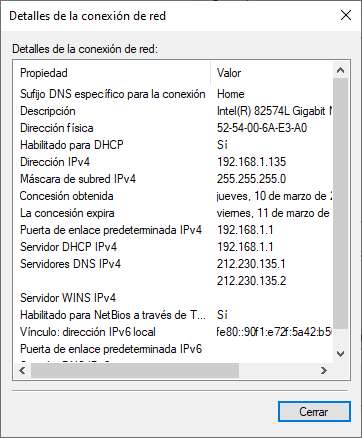
\includegraphics[frame,width=0.4\linewidth]{windows_network_status.png}
    \vspace{-15pt}
\end{center}

Para no dar tantos pasos, si ejecutamos en la terminal \textbf{CMD} el siguiente comando también lo veremos:

\begin{mycode}{Obtener puerta de enlace en Windows}{powershell}{}
C:\Users\ruben> ipconfig

Configuración IP de Windows
Adaptador de Ethernet Instancia de Ethernet 0 2:

Sufijo DNS específico para la conexión. . : Home
Vínculo: dirección IPv6 local. . . : fe80::90f1:e72f:5a42:b50d%7
Dirección IPv4. . . . . . . . . . . . . . : 192.168.1.135
Máscara de subred . . . . . . . . . . . . : 255.255.255.0
Puerta de enlace predeterminada . . . . . : 192.168.1.1
\end{mycode}

Pueden existir equipos sin puerta de enlace, pero no suele ser lo habitual. Esto sucede cuando queremos que equipos puedan ver a otros equipos de la red, pero no puedan comunicarse con el exterior. Suele ser más habitual realizar bloqueos a nivel de firewall.


\hypertarget{nat}{}
\subsection{NAT}
La traducción de direcciones de red, también llamado enmascaramiento de IP o NAT (del inglés \textit{\textbf{Network Address Translation}}), es un mecanismo utilizado por routers que conectan dos (o más) redes para que el paquete que llega a un equipo destino no parezca que llega desde la red de origen.

Vamos a tomar como ejemplo el siguiente esquema que es un ejemplo que podemos entender teniendo en cuenta la conexión de nuestra casa:

\begin{center}
    \vspace{-15pt}
    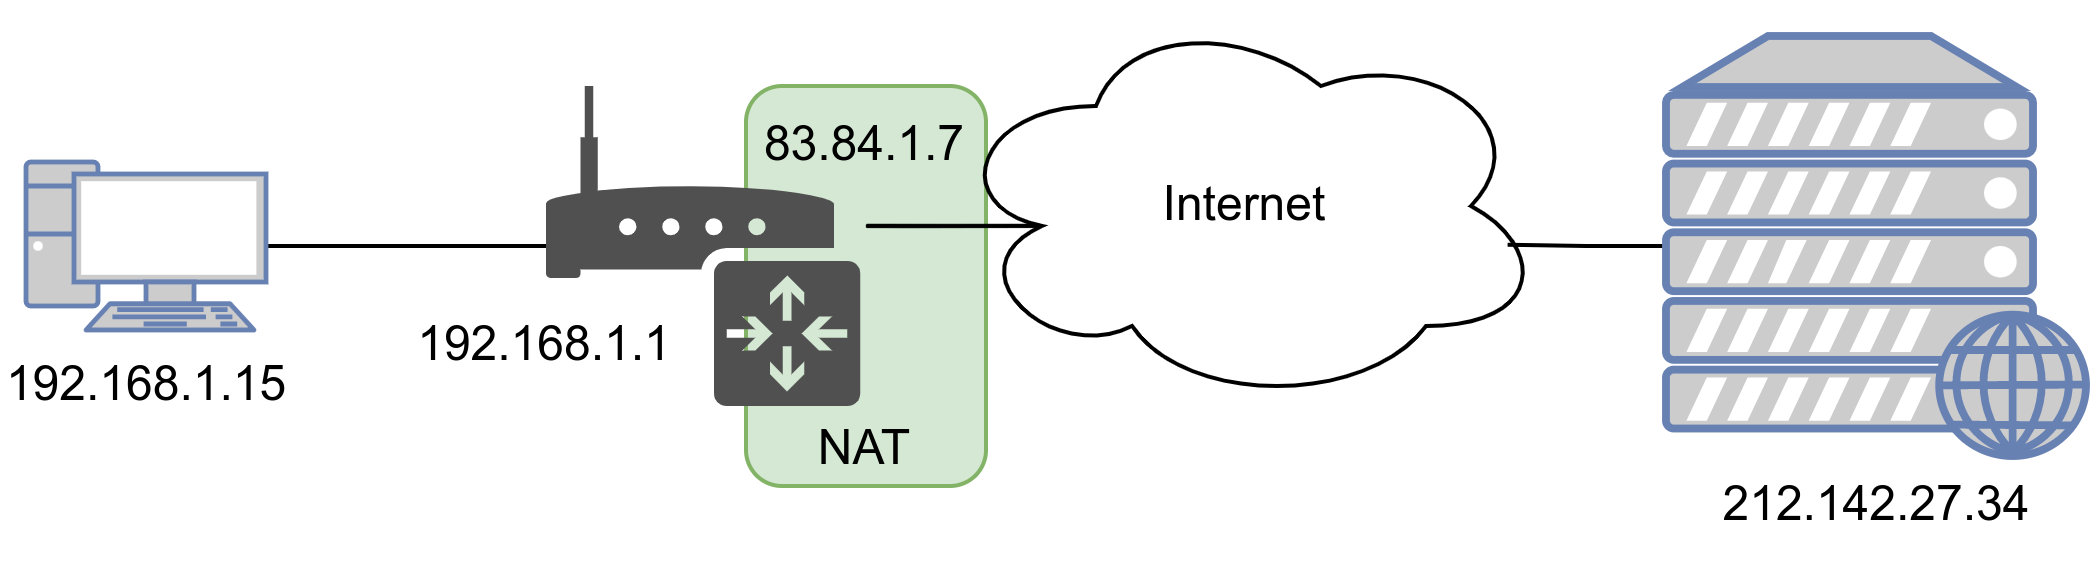
\includegraphics[width=0.8\linewidth]{NAT.png}
    \vspace{-25pt}
\end{center}

En este ejemplo tenemos conectado un equipo con IP 192.168.1.15 al router que tenemos en casa (cuya IP en la LAN es 192.168.1.1). Este router cuenta con una IP pública proporcionada por el ISP para el acceso a internet (83.84.1.7). Cuando nuestro equipo quiere comunicarse con algún equipo que no está en su red, al salir a internet, el router cambia la cabecera del paquete sustituyendo 192.168.1.15 por 83.84.1.7, y de esta manera al servidor remoto (212.142.27.34) el paquete le llega desde una IP pública.

Este es el ejemplo más sencillo y que hacemos uso cada día en casa, pero esto no significa que NAT sólo se realice entre redes públicas y privadas. Lo podemos utilizar entre dos redes públicas o dos redes privadas también.

Las traducciones de dirección se almacenan en una tabla, para recordar qué dirección y puerto le corresponde a cada dispositivo cliente y así saber donde deben regresar los paquetes de respuesta.

Existen distintos tipos de NAT:
\begin{itemize}
    \item \textbf{NAT de sobrecarga}: Varios equipos de la red de origen se traducen por una única dirección de la red de salida. Es el método más habitual (el que realizan nuestros routers en casa).

    \item \textbf{NAT estática}: También conocida como “NAT 1:1”, ya que una dirección IP privada se traduce siempre por una única dirección IP pública, y siempre será la misma. Este método es el habitual cuando queremos tener un servidor en la red interna y queremos que su comunicación con el exterior siempre sea con la misma IP pública

    \item \textbf{NAT dinámica}: Similar al caso anterior, pero en este caso el router contará con una tabla de IPs públicas y se asignará una que esté libre de esta tabla a un equipo interno cuando necesite comunicarse de manera pública. Cuando deje de necesitarlo, la IP se marcará como “libre” y se podrá asignar a otro equipo interno posteriormente.
\end{itemize}


\hypertarget{rutas_estaticas}{}
\subsection{Rutas estáticas}


\subsection{Enrutamiento dinámico}

\subsubsection{BGP (Border Gateway Protocol)}



\section{Administración de routers}









\chapter{Redes virtuales}
Es habitual querer diferenciar distintas redes dentro de una arquitectura de red (para diferenciar departamentos en una empresa, separar servidores de equipos de trabajo, limitar el acceso entre redes, ...) pero eso supone la compra de distintos equipamientos físicos (distintos switches, puntos de acceso ...) que incrementa el coste de nuestra infraestructura.

Para evitar este incremento de precio, podemos hacer uso de las \textbf{VLAN} en nuestros dispositivos de red, ya sea en switches o en routers, que los soporten.

\section{VLAN}
Una VLAN, acrónimo de \textit{virtual LAN} (red de área local virtual), \textbf{es un método para crear redes lógicas independientes dentro de una misma red física}. Varias VLAN pueden coexistir en un único switch físico o en una única red física, y el tráfico estará separado entre distintas VLANs a nivel lógico.

Un equipo de una VLAN no se podrá comunicar con otro equipo de otra VLAN distinta salvo que haya un router que esté conectado en ambas VLANs y que encamine el tráfico de una a la otra. Lo mismo que si fuesen dos redes físicas, como hemos visto hasta ahora.

Las VLANs se diferencian a través de una cabecera extra la cual se añade dentro del encabezado original de la trama (\textbf{capa 2}). Esa cabecera consta de dos partes de 16 bits, siendo los últimos 12 los que correspondan al valor que identificará a la VLAN, y estará comprendido entre 1 y 4095, ya que el 0 está reservado. Esa cabecera indicará que el tráfico está etiquetado o “\textit{\textbf{tagged}}”.

\infobox{Las VLANs se diferencian a través de una cabecera extra la cual se añade dentro del encabezado original de la trama (\textbf{capa 2}).}

A continuación se puede ver cómo se muestra tráfico etiquetado mediante las cabeceras del \textbf{protocolo 802.1Q}:

\begin{center}
    \vspace{-10pt}
    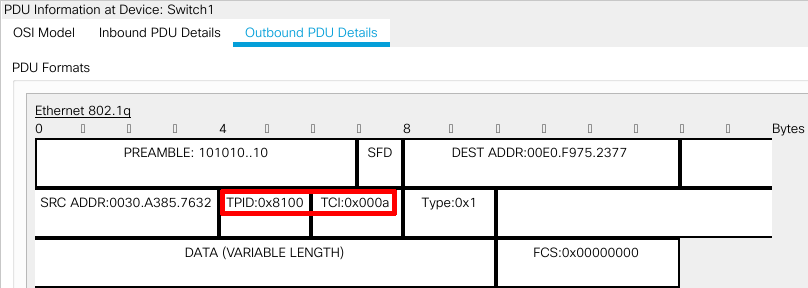
\includegraphics[frame,width=0.9\linewidth]{vlan-tag.png}
    \vspace{-10pt}
\end{center}

\begin{itemize}
    \item \textbf{TPID}: 16 bits en el que el valor  “\textbf{0x8100}” indica que es una trama etiquetada del protocolo \textbf{802.1Q}.
    \item \textbf{TCI}: 16 bits (formando 4 caracteres en hexadecimal):
    \begin{itemize}
        \item \textbf{PCP}: 3 bits que permiten priorizar el tráfico.
        \item \textbf{DEI}: 1 bit, en conjunto con PCP, que permite saber si esta trama se puede descartar en caso de congestión.
        \item \textbf{VID}: \textit{VLAN IDentificator}, 12 bits ($2^{12} = 4096$). En este caso los últimos 3 caracteres hexadecimales “00A” que indica que es la VLAN 10.
    \end{itemize}
\end{itemize}

Hay que tener en cuenta que aunque existe el límite de 4096 VLANs, algunos switches tienen una limitación de un número menor de VLANs activas. Es decir, puedes crear VLANs con el dígito que quieras (hasta 4095), pero quizá sólo te dejan crear 16 VLANs. Ejemplo de la limitación del número de VLANs que puede haber activas en switches “\href{https://www.cisco.com/c/dam/en/us/products/collateral/switches/small-business-100-series-unmanaged-switches/data_sheet_c78-634369_Spanish.pdf}{Cisco de la serie 200 Cisco Small Business}”:

\begin{table}[H]
    \centering
    \begin{tabular}{|L{0.1\linewidth}|L{0.84\linewidth}|}
        \tbody
        VLAN & Compatibilidad con hasta \textbf{256 VLAN simultáneas} (de 4096 ID de VLAN). \textbf{16 VLAN compatibles en SG200-08 y SG200-08P}. VLAN basadas en puertos y en etiquetas 802.1Q
        \\ \hline
        VLAN de voz & El tráfico de voz se asigna automáticamente a una VLAN específica de voz y se trata con los niveles apropiados de QoS
        \\ \hline
    \end{tabular}
    \vspace{-15pt}
\end{table}

Como se puede apreciar, en este modelo de Switch, el límite es de 256 VLAN activas (aunque se puede elegir el ID de la VLAN de las 4096 posibles), y de “sólo” 16 VLANs en el modelo de 8 bocas ethernet de esa serie.


\subsection{Diferencia de arquitecturas con y sin VLANs}
Para que quede más claro lo explicado hasta ahora, vamos a analizar una misma infraestructura de red separada a nivel físico y separada a nivel lógico mediante VLANs.

\subsubsection{Arquitectura sin VLAN}
En una arquitectura de red sin VLANs tendríamos que tener tantos switches como sean necesarios para realizar una separación física de las redes. Estos switches estarán conectados a un router que será el encargado de encaminar el tráfico entre las redes. La separación física de redes es más cara ya que se necesita más hardware y es posible que los switches estén infrautilizados.

\begin{center}
    \vspace{-15pt}
    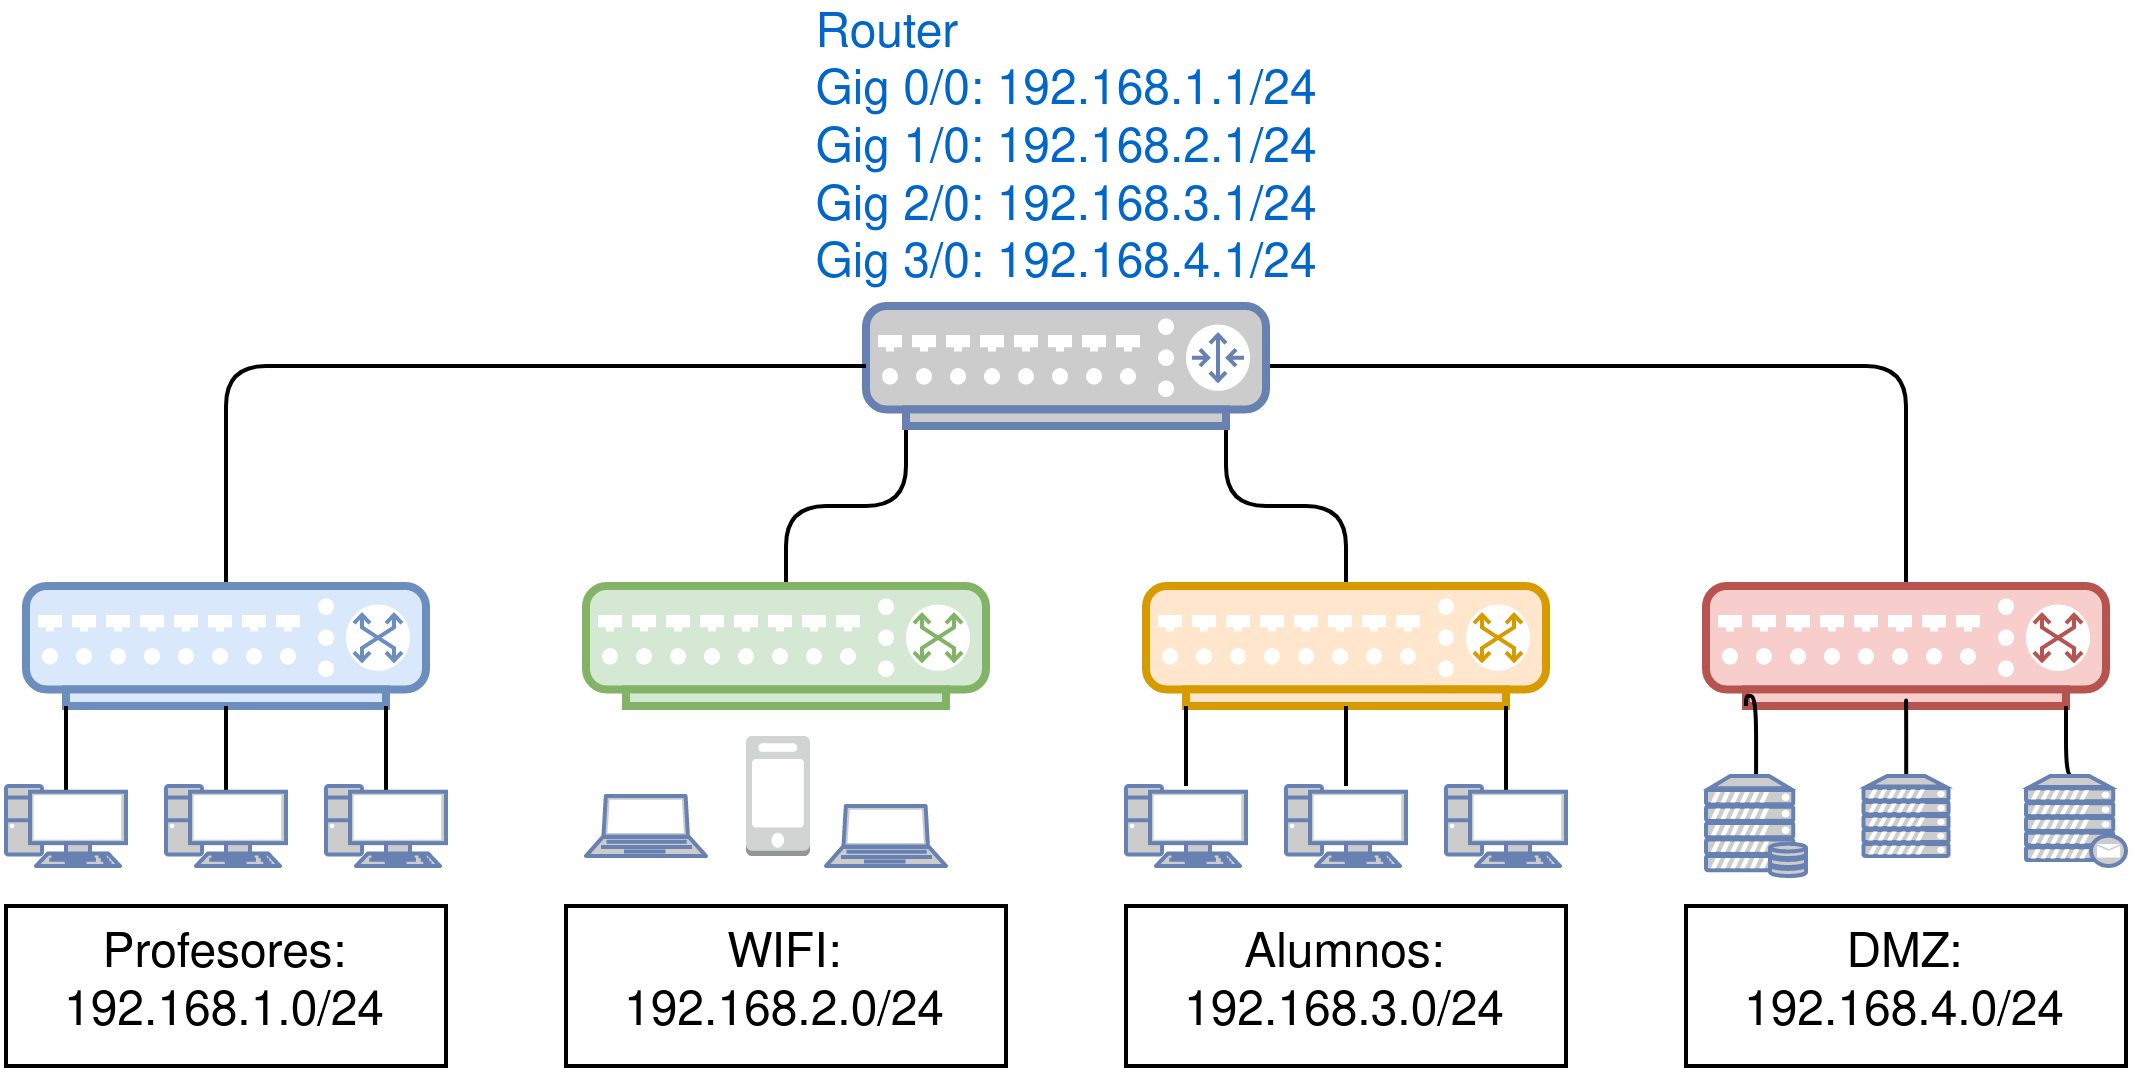
\includegraphics[width=0.8\linewidth]{red-sin-vlan.png}
    \vspace{-15pt}
\end{center}

Se puede observar una arquitectura en la que un router actúa de intermediación en una red en la que existen 4 redes separadas físicamente mediante distintos switches. Si en una red existen pocos dispositivos, el switch de esa red estará infrautilizado. Si por el contrario necesitamos ampliar alguna de las redes, deberemos añadirle un switch en cascada en la red correspondiente, pero aún así ese nuevo switch podría estar infrautilizado.


\subsubsection{Arquitectura con VLANs}

En una arquitectura con \textbf{VLAN}s, tendremos un router que estará conectado a un switch mediante un enlace \hyperlink{puerto_trunk}{trunk}, y en este switch se configurará cada interfaz en modo \hyperlink{puerto_access}{access} teniendo en cuenta el dispositivo que se vaya a conectar a dicha interfaz. En caso de necesitar ampliar las redes, se hará uso de las interfaces no utilizadas, y en caso de no haber más, el switch se podría expandir añadiendo uno nuevo y \hyperlink{stack_switches}{creando un stack} entre ellos.

\begin{center}
    \vspace{-15pt}
    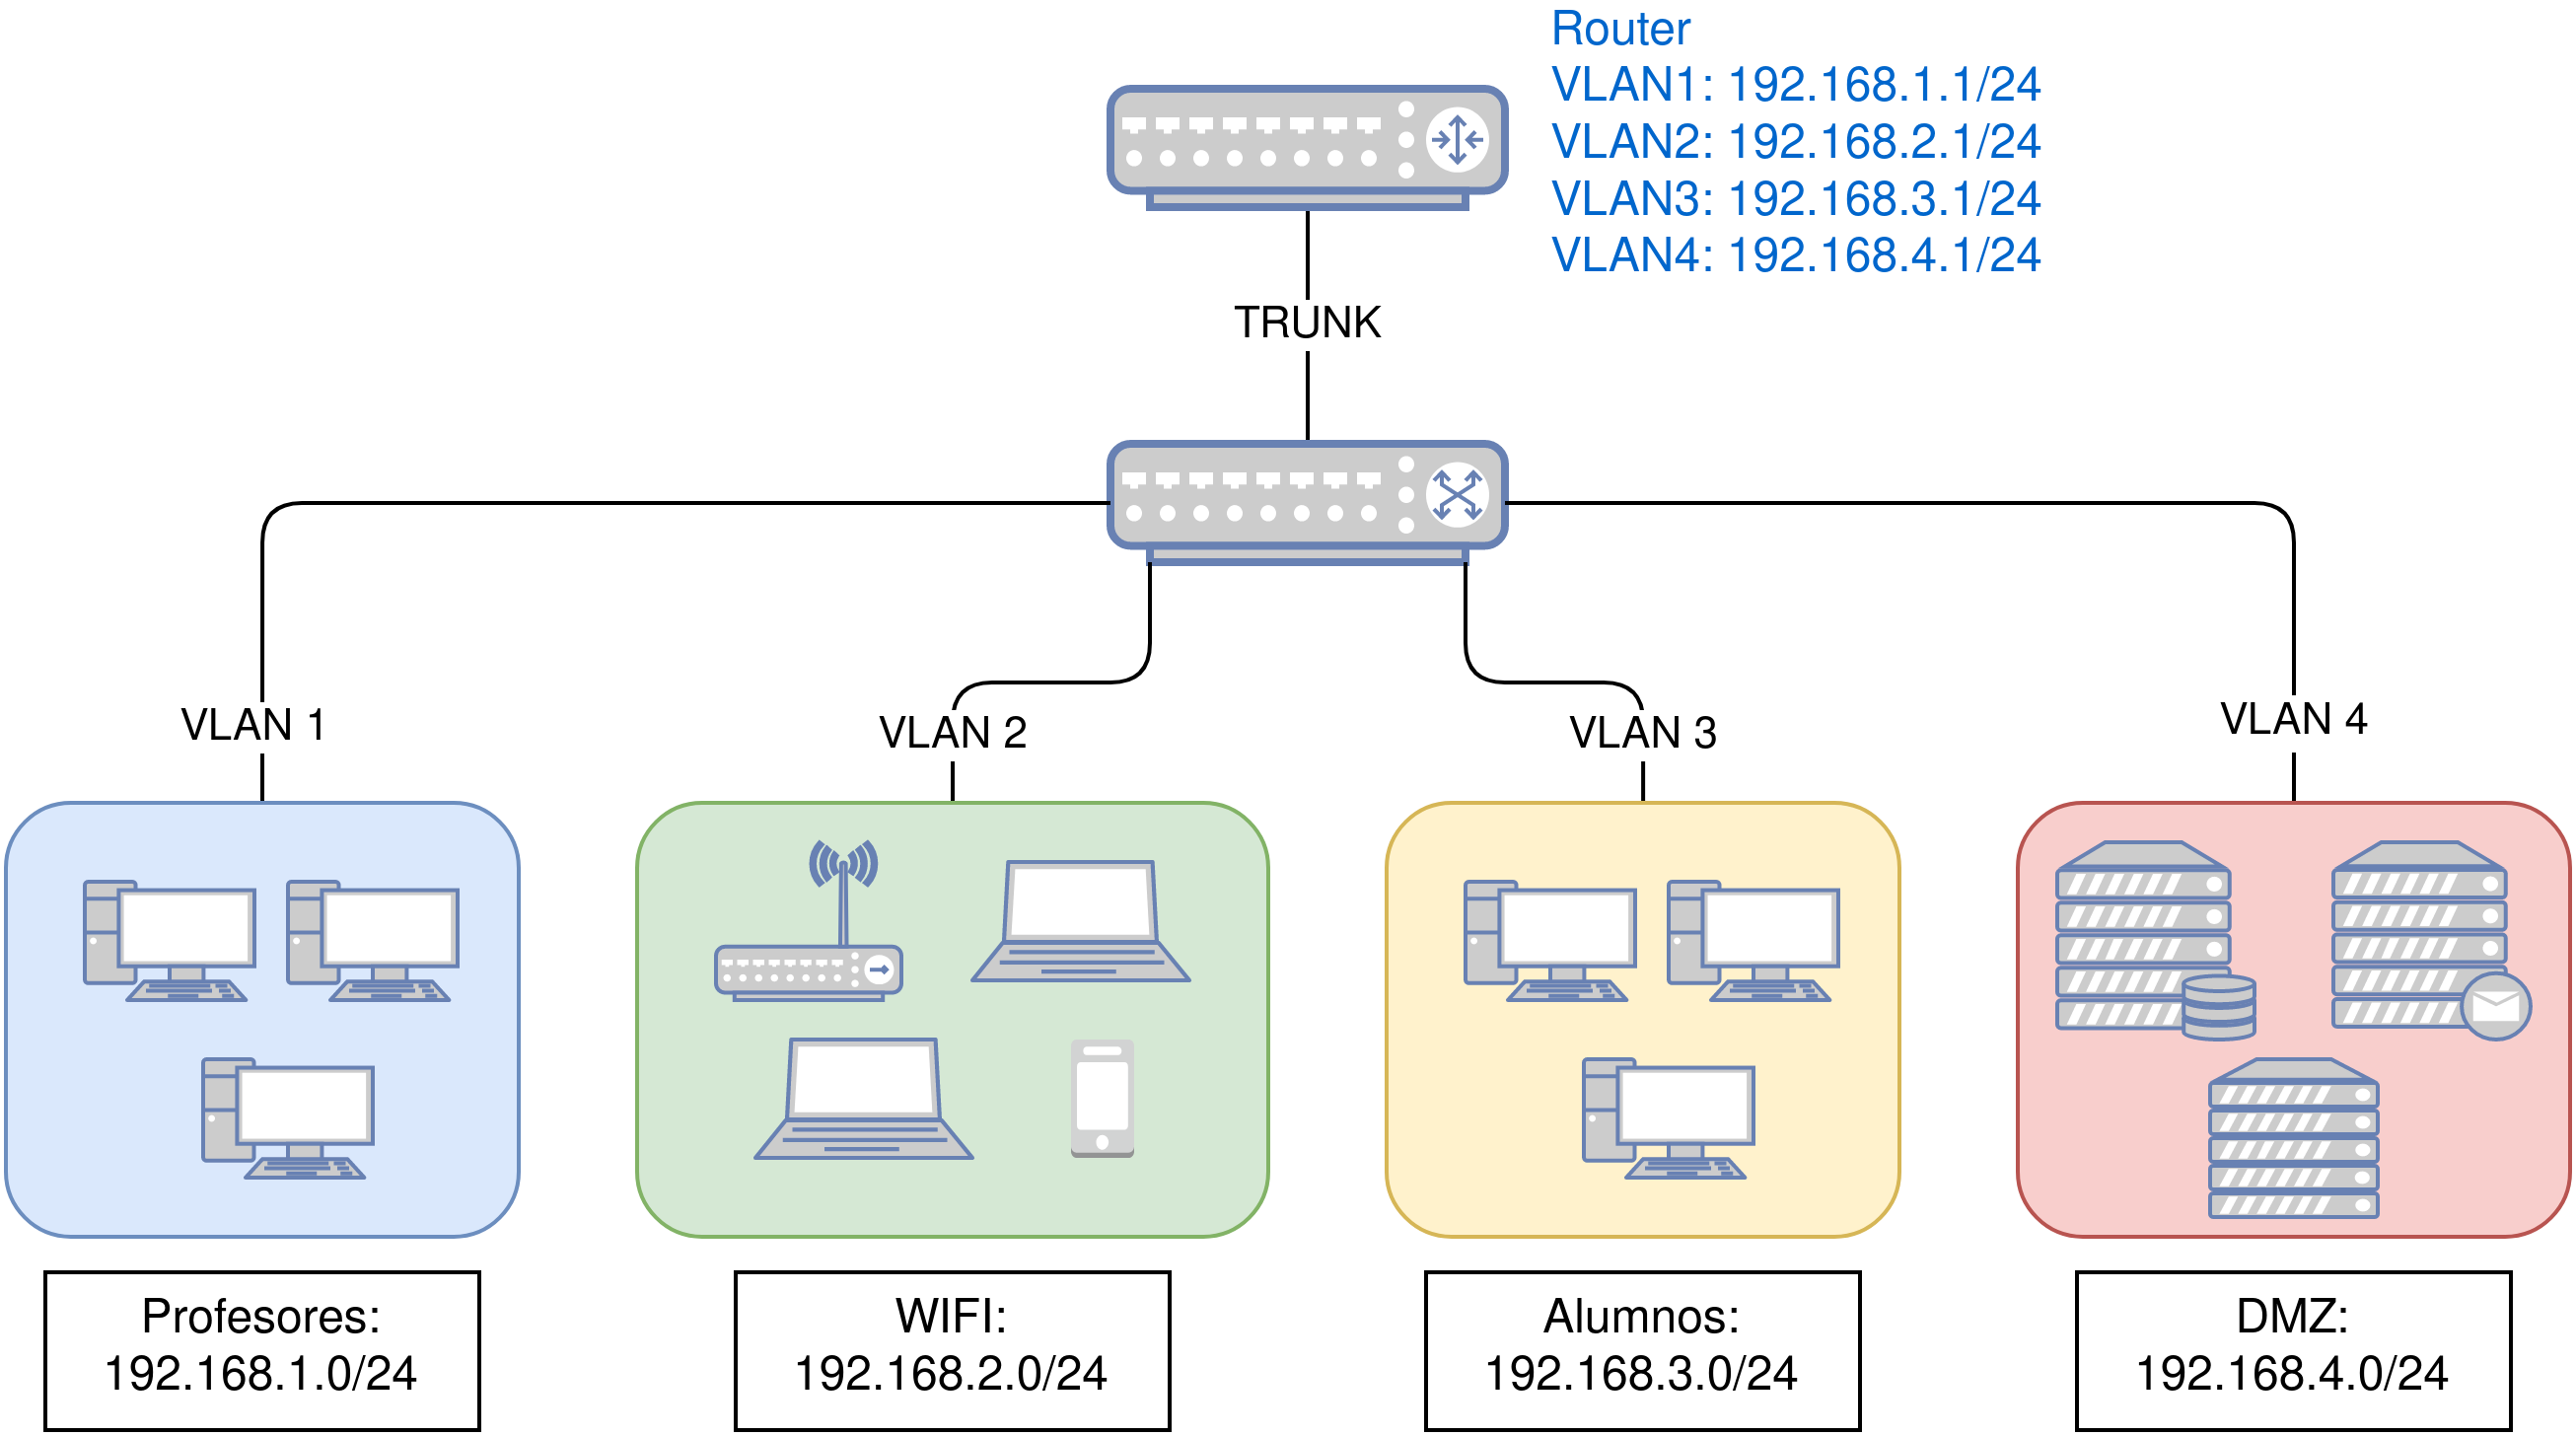
\includegraphics[width=0.8\linewidth]{red-con-vlan.png}
    \vspace{-15pt}
\end{center}

\section{VLANs en Switches}

En los switches se pueden realizar distintas configuraciones teniendo en cuenta las VLANs que vayamos a utilizar y la arquitectura de red que tengamos:

\begin{itemize}
    \item \textbf{VLAN por defecto en el switch}: Es la VLAN en la que trabajará el switch. Por defecto suele ser la \textbf{VLAN 1}. El tráfico por defecto va en esa VLAN y para ir por cualquier otra VLAN el tráfico deberá estar “\textit{tagged}” (etiquetado).

    \hypertarget{puerto_trunk}{}
    \item \textbf{Puerto en modo “\textit{trunk}”}: Normalmente utilizado para comunicación entre distintos switches y/o routers. A este enlace “\textbf{\textit{trunk}}” (o troncal, o tronco) se le asigna una VLAN por defecto y las VLANs “\textbf{tagged}” permitidas que pasarán por él. Los switches sabrán a qué VLAN pertenece cada trama observando la etiqueta VLAN de la capa 2.

    El tráfico que \textbf{entra} en esta boca, si no está etiquetado estará en la VLAN por defecto. Si está etiquetado en una VLAN permitida se permitirá el tráfico.

    El tráfico que \textbf{sale} de esta boca saldrá de la misma manera con la que llegó a él (sin etiquetar o etiquetado con la VLAN que sea). El equipo que reciba esta trama tendrá que lidiar con el tráfico recibido (ya sea etiquetado o no).

    \hypertarget{puerto_access}{}
    \item \textbf{Puerto en modo “\textit{access}”}: La boca del switch se define en modo “access” (o “acceso”) y se le asigna una \textbf{única VLAN} a la misma.

    Este tipo de configuraciones suele ser utilizada para conectar equipos en los que no podemos etiquetar VLANs en origen (impresoras por ejemplo), o nos resulte tedioso la configuración de la misma, pero queremos asegurar que su tráfico viaje por una VLAN.

    El \textbf{tráfico que entra} en esta boca, a partir de ese momento \textbf{se le añadirá la cabecera de la VLAN a la trama} convirtiéndose en tráfico “tagged”.

    Si el \textbf{tráfico sale} de una boca en modo “access” se quitará la cabecera VLAN, por lo que \textbf{al equipo remoto le llegará el tráfico sin estar “tagged”}.

\end{itemize}

Teniendo en cuenta lo explicado previamente, se puede observar en el siguiente dibujo en el que aparecen varios switches, configurados con distintas bocas en modo \textbf{access} y otras en modo \textbf{trunk}. Como se puede ver, las bocas que comunican los distintos dispositivos (switches con switches y switch con router) están configuradas en modo TRUNK, y en ellas se permiten varias VLANs.

Las interfaces que sólo tienen un color, están configuradas en modo \textbf{access} con una VLAN. Los interfaces en blanco no están configurados (ya que usan la VLAN por defecto, en este caso la VLAN 1). Para que el router pueda enrutar las distintas redes, le tendrán que llegar a través de un enlace configurado en modo \textbf{trunk}.
\textbf{}

\begin{center}
    \vspace{-10pt}
    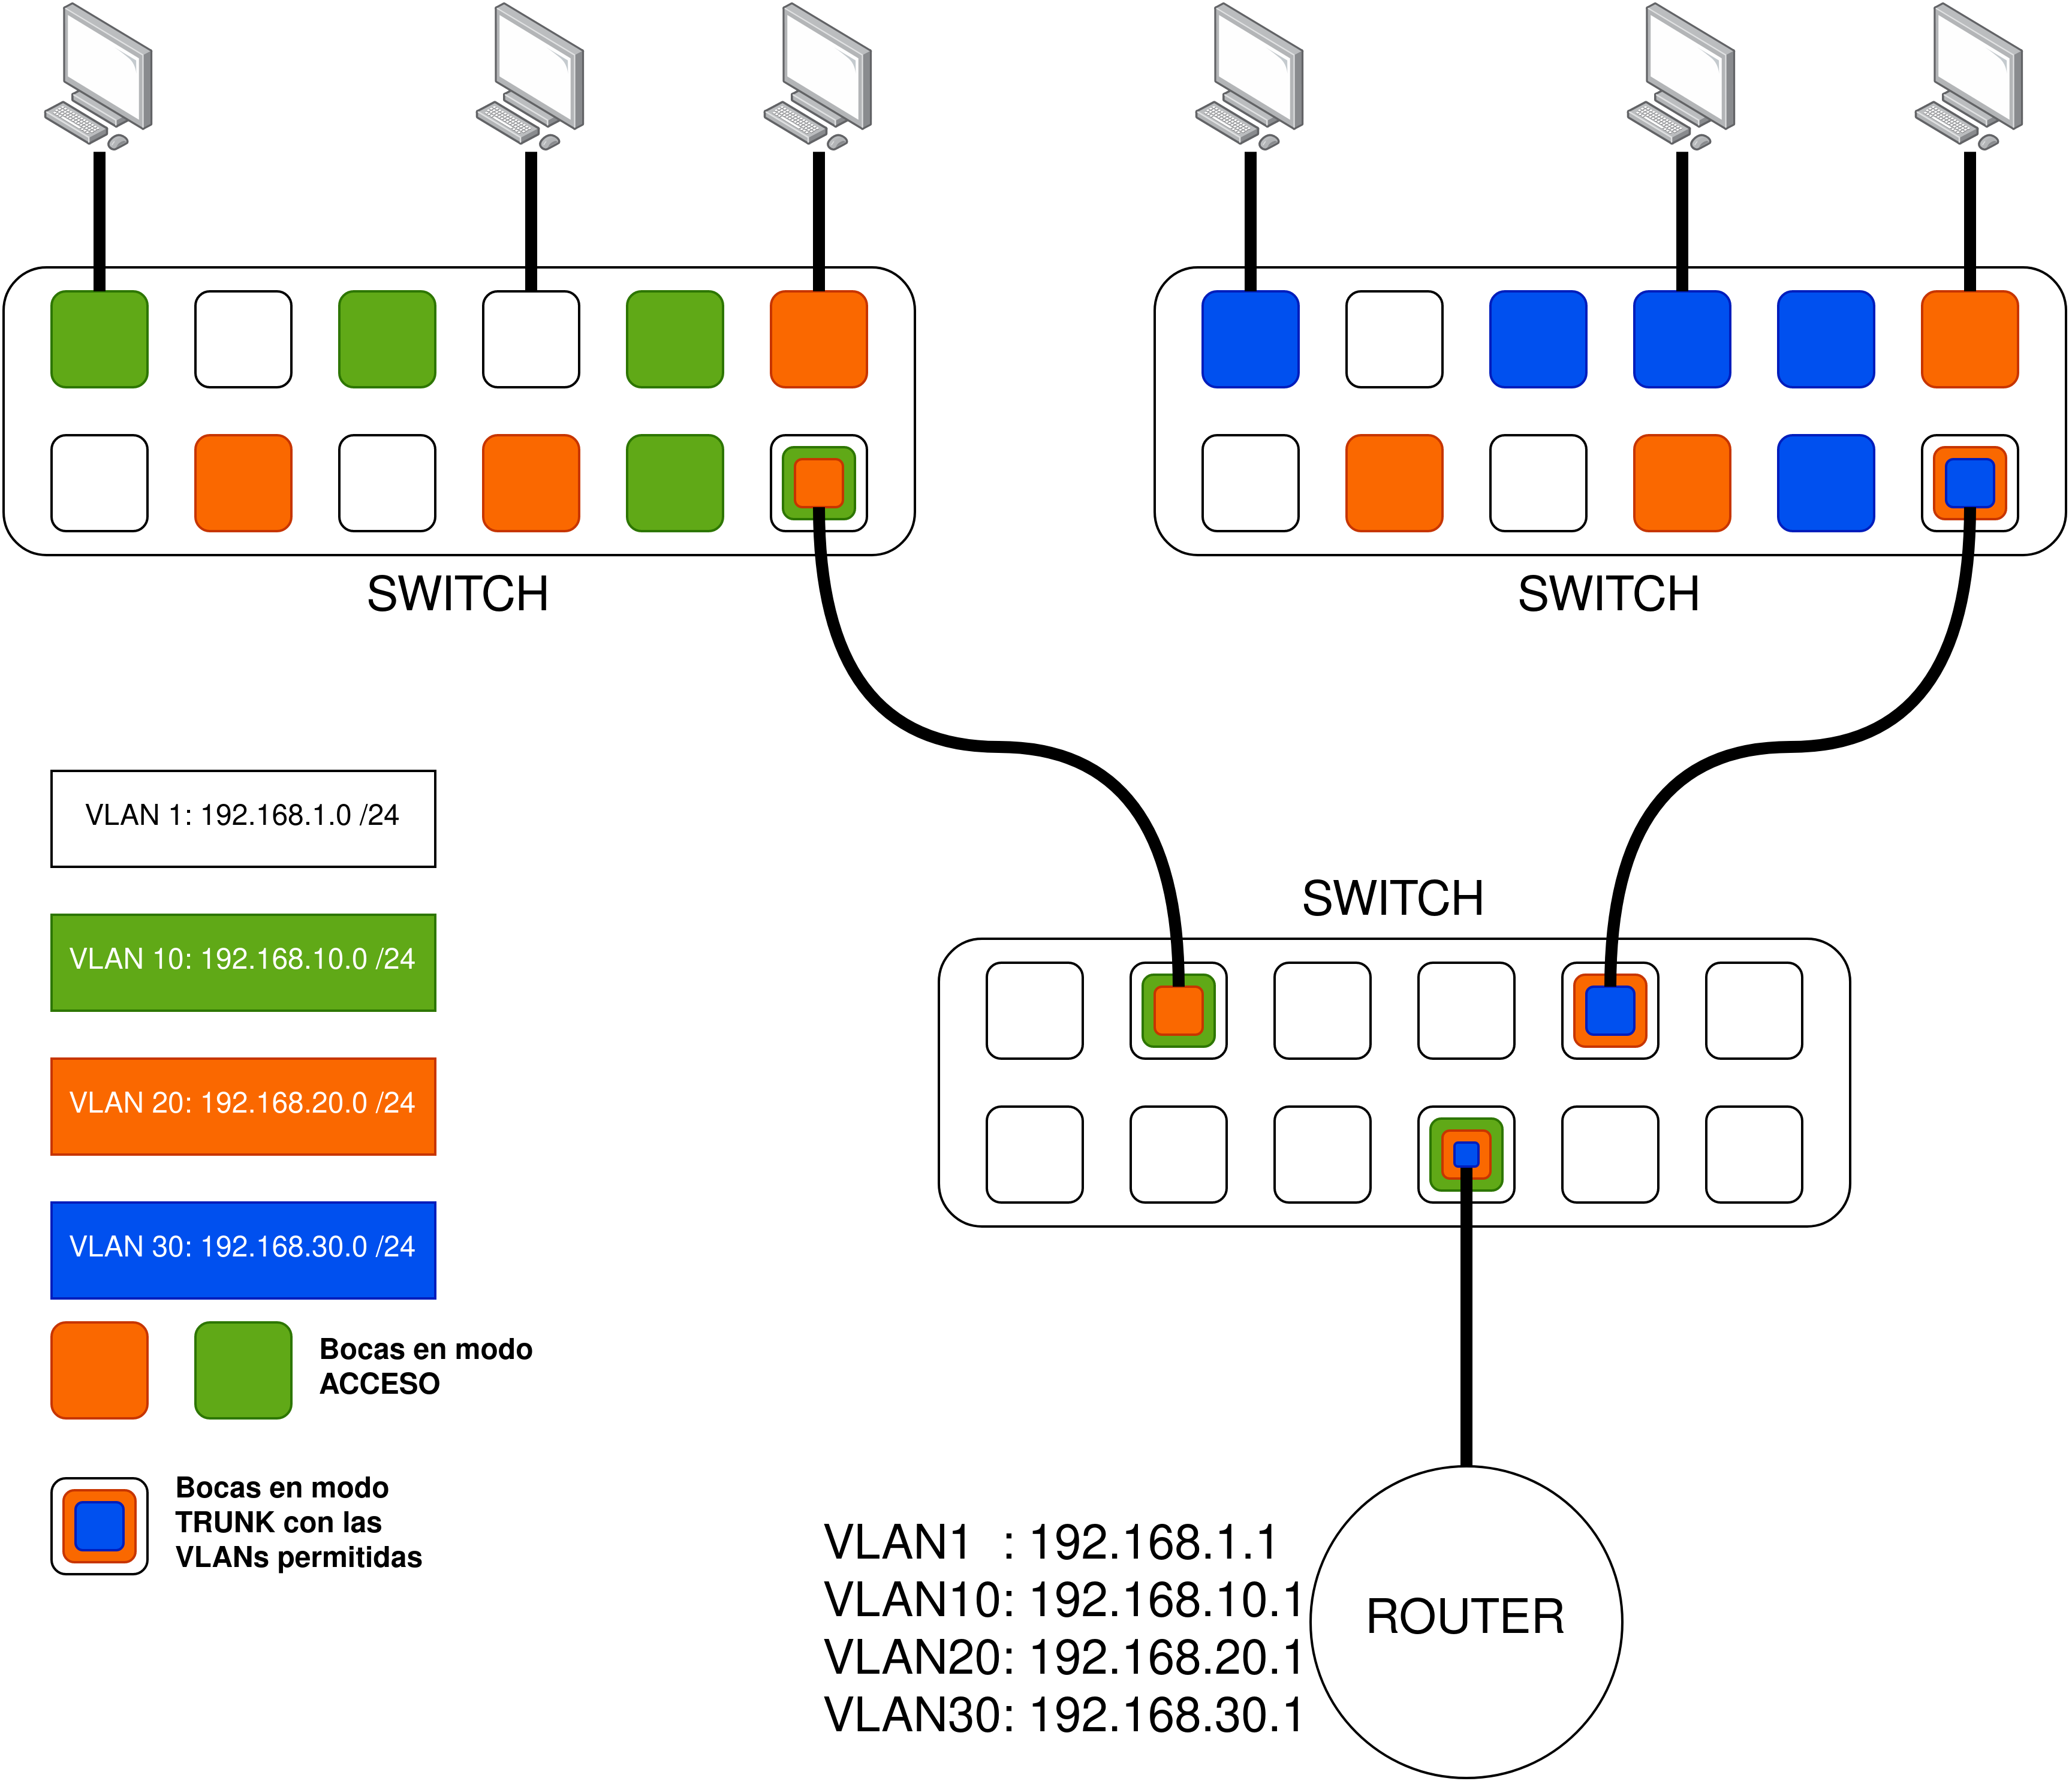
\includegraphics[width=0.9\linewidth]{switch_configuracion_access_trunk.png}
    \vspace{-10pt}
\end{center}


\subsection{Crear VLAN}
Para crear una VLAN primero deberemos identificar el identificador, y luego suele ser recomendable darle un nombre identificativo.

\begin{mycode}{Crear VLAN}{powershell}{}
Switch(config)# vlan 10
Switch(config-vlan)# name Profesores
\end{mycode}

\subsection{Añadir IP en una VLAN}
En caso de necesitarlo, se podrá añadir una IP a cada nueva vlan que se haya creado, tal como se hace con la VLAN 1, pero eligiendo la VLAN correspondiente.

\begin{mycode}{Añadir IP a la VLAN}{powershell}{}
switch(config)# interface vlan10
switch(config-if)# ip address 10.10.0.254 255.255.255.0
switch(config-if)# no shutdown
\end{mycode}

\subsection{Listar tabla de VLAN}
El siguiente comando nos muestra la base de datos interna de VLANs que tiene el switch, indicando el estado y un pequeño resumen de en qué bocas está activa. Hay que tener en cuenta que no nos indica en qué modo está configurada dicha VLAN en cada interfaz, por lo que deberemos comprobarlo mirando detalladamente la configuración completa.

\begin{mycode}{Listar la tabla de VLAN}{powershell}{}
Switch# show vlan

VLAN    Name            Status    Ports
---- ------------------ --------- --------
1    default            active    Gig1/1
10   profesores         active    Gig0/1
20   alumnos            active
...
\end{mycode}

También hay que tener en cuenta que aunque un interfaz esté configurado con una VLAN, si no aparece en la base de datos, es como si no existiese.

\subsection{Configurar interfaz con VLAN en acceso}
Para configurar un interfaz en modo \textbf{\textit{access}} tendremos que elegir primero el interfaz y después elegir el modo a configurar y para qué VLAN. Es importante haber creado primero la VLAN.
\begin{mycode}{Configurar interfaz en modo trunk}{powershell}{}
Switch(config)# interface GigabitEthernet 0/1
Switch(config-if)# switchport mode access
Switch(config-if)# switchport access vlan 10
\end{mycode}


\subsection{Configurar interfaz con VLAN en trunk}
Para configurar un interfaz en modo \textbf{\textit{trunk}} tendremos que elegir primero el interfaz y después elegir el método de configuración:

\begin{mycode}{Configurar interfaz en modo trunk}{powershell}{}
Switch (config)# interface GigabitEthernet 1/1
Switch(config-if)# switchport mode trunk
Switch(config-if)# switchport trunk allowed vlan  ???
\end{mycode}

Donde “???” pueden ser varias opciones:
\begin{itemize}
    \item \textbf{add}: add VLANs to the current list
    \item \textbf{all}: all VLANs
    \item \textbf{except}: all VLANs except the following
    \item \textbf{none}: no VLANs
    \item \textbf{remove}: remove VLANs from the current list
\end{itemize}
Podemos poner la VLAN por defecto en una boca en modo trunk con:

\begin{mycode}{Poner vlan por defecto en un trunk}{powershell}{}
Switch(config-if)# switchport trunk native vlan 10
\end{mycode}


\subsection{VLANs en Routers}
En los routers, las VLANs van asociadas a una interfaz física. Al añadir una VLAN, se crea una interfaz “virtual”, y dentro se le indica que va a ser de tipo “\textbf{encapsulation dot1Q}” y la VLAN que va a usar. Después, se le configura la IP como si fuera una interfaz normal. Como ejemplo para la VLAN 20:

\begin{mycode}{Crear VLAN 20 en Router y configurar una IP}{powershell}{}
Router(config)# interface GigabitEthernet0/0.20
Router(config-if)# encapsulation dot1Q 20
Router(config-if)# ip address 192.168.20.1 255.255.255.0
\end{mycode}




\subsection{VLANs en servidores/ordenadores}
El tráfico que “sale” de un servidor/ordenador, por defecto, no está etiquetado con ninguna VLAN. En caso de que queramos que el tráfico saliente salga con una VLAN etiquetada, tendremos que configurar el interfaz de red para que funcione con dicha VLAN.



\section{Protocolo VTP}
VTP, o \textbf{VLAN Trunk Protocol}, es un protocolo que nos permite configurar y administrar VLANs en equipos Cisco de manera centralizada. De esta manera conseguimos simplificar la tarea cuando tenemos una red en la que disponemos de muchas VLANs

El protocolo funciona en modo  servidor-cliente, por lo tanto debemos configurar un switch en modo servidor, que será en el que realizaremos la administración de las VLANs, que posteriormente serán propagadas por los switches que son clientes VTP y que pertenecen al mismo dominio.


\warnbox{La conexión entre switches debe estar en modo \textbf{trunk} para que el protocolo funcione de manera correcta.}

\subsection{Configurar switch como VTP Server}
Es tan fácil como elegir el modo servidor del protocolo VTP, indicar un dominio de propagación y una contraseña para el mismo.

\begin{mycode}{Crear configuración como VTP Server}{powershell}{}
Switch(config)# vtp mode server
Switch(config)# vtp domain instituto
Switch(config)# vtp password 1234
\end{mycode}

\subsection{Configurar switch como VTP Client}
Similar al caso anterior, pero esta vez eligiendo que queremos que el switch sea cliente:

\begin{mycode}{Crear configuración como VTP Client}{powershell}{}
    Switch(config)# vtp mode client
    Switch(config)# vtp domain instituto
    Switch(config)# vtp password 1234
\end{mycode}

\subsection{Ver estado de VTP}
Para comprobar el estado del servicio VTP, tanto en un switch que sea \textit{server} o \textit{client}:

\begin{mycode}{Ver configuración de estado de VTP}{powershell}{}
Switch# show vtp status

VTP Version                     : 2
Configuration Revision          : 2
Maximum VLANs supported locally : 255
Number of existing VLANs        : 7
VTP Operating Mode              : Server
VTP Domain Name                 : instituto
VTP Pruning Mode                : Disabled
VTP V2 Mode                     : Disabled
VTP Traps Generation            : Disabled
MD5 digest                      : 0x68 0x70 0x3B 0xF0 0x14 0xC8 0xF7 0xE9
Configuration last modified by 0.0.0.0 at 3-1-93 00:11:38
Local updater ID is 0.0.0.0 (no valid interface found)
\end{mycode}

Y nos ofrece un resumen del estado del mismo.



\chapter{Alta Disponibilidad en sistemas de red}
La \hyperlink{altadisponibilidad}{Alta Disponibilidad} en una arquitectura de red es vital si queremos asegurar el acceso a otras redes o servicios. Para ello podemos hacer uso de distintas tecnologías que nos ayudarán a conseguirlo.



\section{Agregación de enlaces: Etherchannel / LACP}
La agregación de enlaces consiste en combinar (agregar) varias conexiones en paralelo para aumentar el \textit{\textbf{throughput}} (la tasa de transferencia) que conseguiría una única conexión. Un grupo de agregación de enlaces (\textbf{LAG}, de \textit{Link Aggregation Group}) combina una serie de puertos físicos de manera que se consigue una única ruta con más ancho de banda que un único enlace.

A lo largo de los años ha habido distintos estándares para la creación de agregación de enlaces. El último es el conocido como \textbf{LACP} (\textit{Link Aggregation Control Protocol}), que provee un método para controlar la unión de varios puertos físicos formando un único canal lógico. LACP permite negociar automáticamente la unión entre dispositivos mediante el envío de paquetes LACP al otro dispositivo.
LACP permite el modo:

\begin{itemize}
    \item \textbf{activo}: Habilita LACP de manera incondicional. Esto puede hacer que si en las bocas que están habilitadas en modo LACP se conecta algo que no está configurado para ello, no funcione de manera correcta
    \item \textbf{pasivo}: Habilita LACP sólamente cuando se detecta un dispositivo configurado con LACP
\end{itemize}

Como ya se ha comentado, la finalidad es la de unir distintas conexiones para aumentar la tasa de transferencia, y esto no sólo se puede realizar entre switches, si no que también se puede realizar entre un switch y un servidor.

A continuación podemos ver cómo sería un sistema LACP entre dos switches.

\begin{center}
    \vspace{-10pt}
    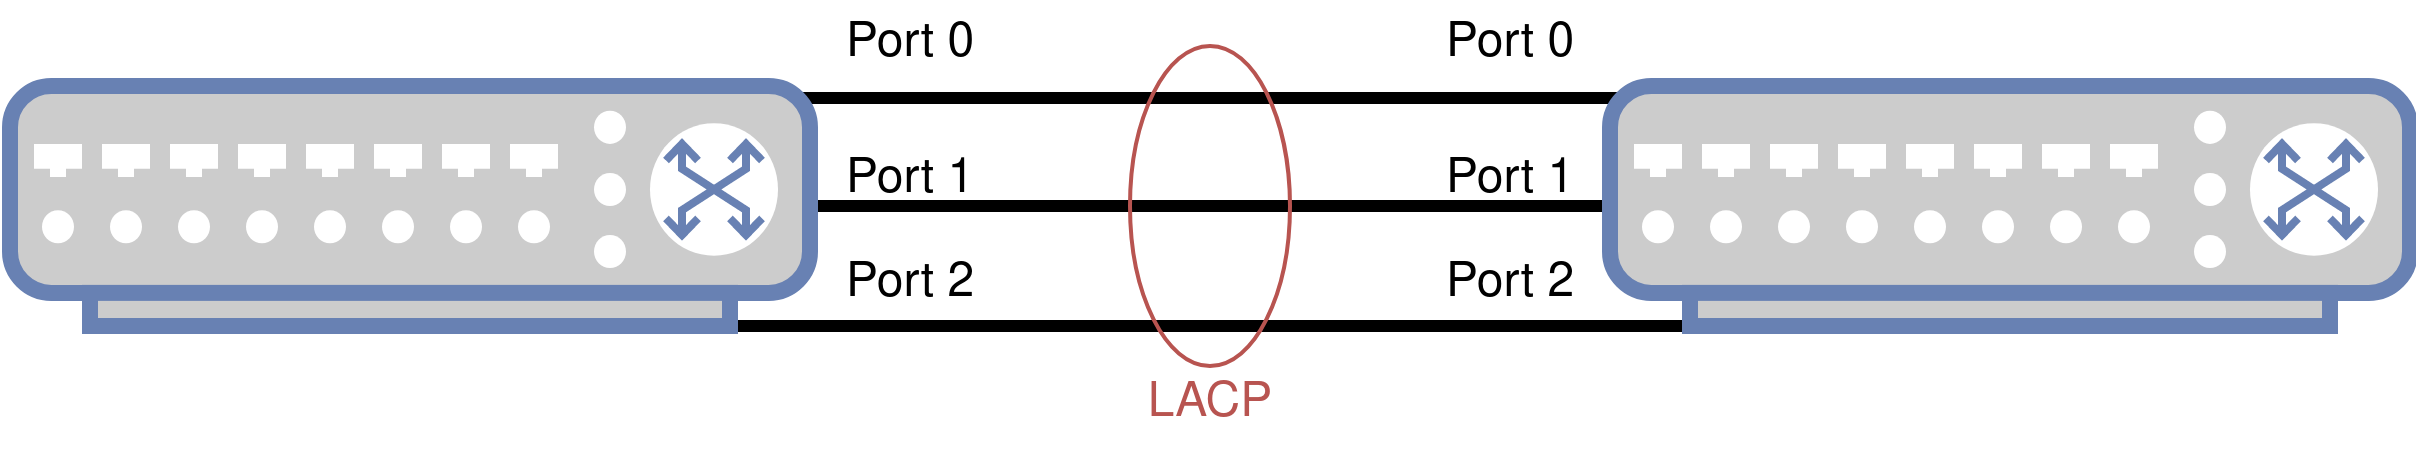
\includegraphics[width=0.7\linewidth]{LACP-switches.png}
    \vspace{-10pt}
\end{center}

Y aquí podemos ver cómo sería una agregación de enlaces entre un switch y un servidor (ya que en un servidor también podemos realizar la agregación de enlaces).

\begin{center}
    \vspace{-10pt}
    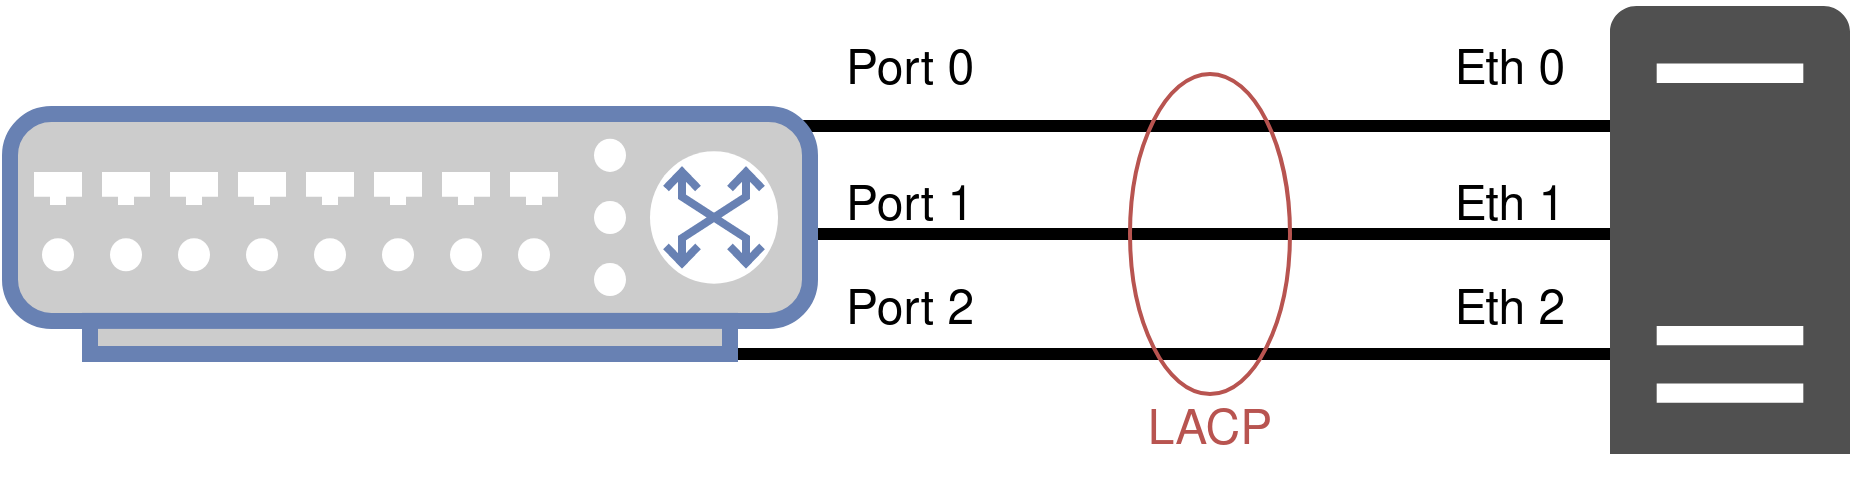
\includegraphics[width=0.6\linewidth]{LACP-switch-server.png}
    \vspace{-10pt}
\end{center}


\subsection{Configurar Etherchannel en Switches}
Antes de realizar ninguna configuración, debemos pensar qué interfaces queremos combinar en una agregación formada por el protocolo LACP.

Para realizar la configuración, deberemos entrar en cada interfaz y añadirlo a un channel-group (siendo el identificador entre el número 1 y el 6) y activar el protocolo a usar:


\begin{mycode}{Añadir interfaces a un \textbf{LAG}}{powershell}{}
Switch(config-if)# channel-group 1 mode active
Switch(config-if)# channel-protocol lacp
\end{mycode}

Cuando se crea un grupo de agregación de enlaces se crea un nuevo interfaz llamado “\textbf{Port-Channel}” (abreviado como “\textbf{Po}”). Es decir, si hacemos la agregación de enlaces con las bocas “0/1” y “1/1” del switch para generar un “channel-group 1”, el switch generará una boca nueva llamada “Port-Channel 1”, la cual podrá ser configurada para hacer lo que necesitemos. En Packet Tracer se pueden tener hasta 6 port-channels:

\begin{mycode}{Configurar Port-Channel 1 en modo \textbf{trunk}}{powershell}{}
switch(config)# interface Port-Channel 1
switch(config-if)# switchport mode trunk
\end{mycode}


Para poder ver el estado del etherchannel/agregación de enlaces:

\begin{mycode}{Ver el estado de los etherchannels}{powershell}{}
Switch# show etherchannel summary

Flags:  D - down        P - in port-channel
I - stand-alone s - suspended
H - Hot-standby (LACP only)
R - Layer3      S - Layer2
U - in use      f - failed to allocate aggregator
u - unsuitable for bundling
w - waiting to be aggregated
d - default port

Number of channel-groups in use: 2
Number of aggregators:           2

Group  Port-channel   Protocol   Ports
------+-------------+-----------+--------------------
1      Po1(SU)           LACP     Gig0/1(P) Gig1/1(P)
2      Po2(SU)           LACP     Gig2/1(P) Gig3/1(P)
\end{mycode}

En este ejemplo, el switch tiene dos agregaciones de enlaces creadas, dos port-channels:
\begin{itemize}
    \item \textbf{Po1}: Tiene configurados los interfaces: Gig 0/1 y Gig 1/1.
    \item \textbf{Po2}: Tiene configurados los interfaces: Gig 2/1 y Gig 3/1.
\end{itemize}

\warnbox{Cada interfaz de cada agregación de enlaces tiene que aparecer con un “\textbf{(P)}”.
    Eso significa que pertenece al port-channel y está correcto.
}


\hypertarget{stack_switches}{}
\section{Stack de switches}

\begin{wrapfigure}{r}{0.36\linewidth}
    \centering
    \vspace{-40pt}
    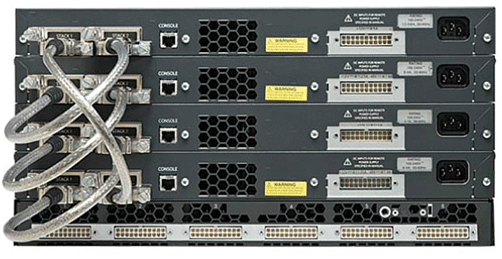
\includegraphics[width=\linewidth]{stack_fisico.png}
    \vspace{-32pt}
    \captionof{figure}{Stack mediante cables especiales}
    \vspace{-30pt}
\end{wrapfigure}
De manera resumida, es la configuración aplicada a varios switches para que actúen como uno sólo. Esto se realiza mediante la interconexión de los switches (formando un anillo) a través de unos puertos especiales o unas conexiones habilitadas para ello.

Tras la realización del “stackado” de switches las ventajas que obtendremos son muy significativas:

\begin{itemize}
    \item Podremos configurar todas las bocas del conjunto de todos los switches que lo forman desde un único punto central (ya sea mediante el CLI o mediante la web de gestión).
    \item Tendremos redundancia en las comunicaciones.
    \item Permite escalar el tamaño de las comunicaciones y podríamos añadir más switches en un momento dado (algunas marcas permiten 12 switches en un mismo stack).
\end{itemize}

Hay que tener en cuenta que no todos los switches permiten realizar un stack de switches, por lo que tendríamos que asegurarnos que si vamos a necesitar esta funcionalidad, a la hora de comprar los switches lo soporten.

\begin{center}
    \vspace{-10pt}
    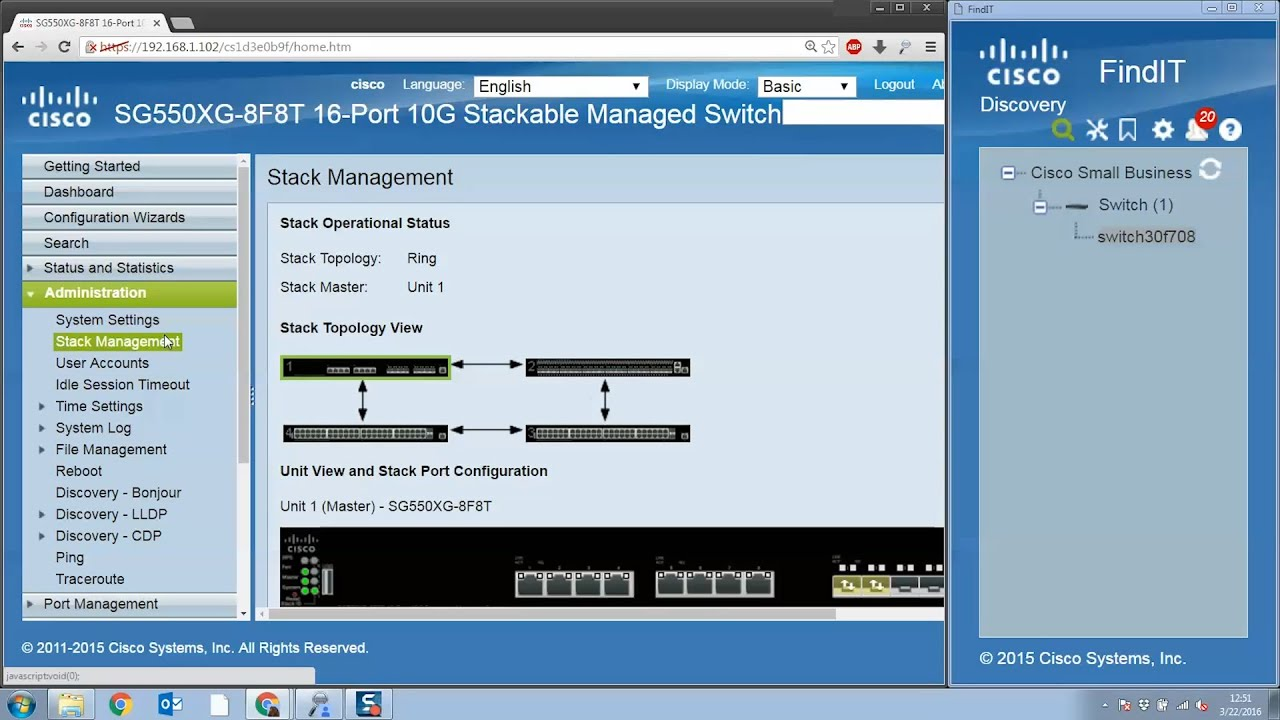
\includegraphics[frame,trim={5 255 572 75},clip,width=0.6\linewidth]{stack_cisco.jpg}
    \vspace{-10pt}
\end{center}


\subsection{Integración de Stack y LACP}
Si realizamos la combinación de configuraciones de Stack de switches junto con LACP con servidores, nos aseguraremos de tener una Alta Disponibilidad real en lo que se refiere a comunicaciones.

Veamos el siguiente dibujo:


\begin{center}
    \vspace{-10pt}
    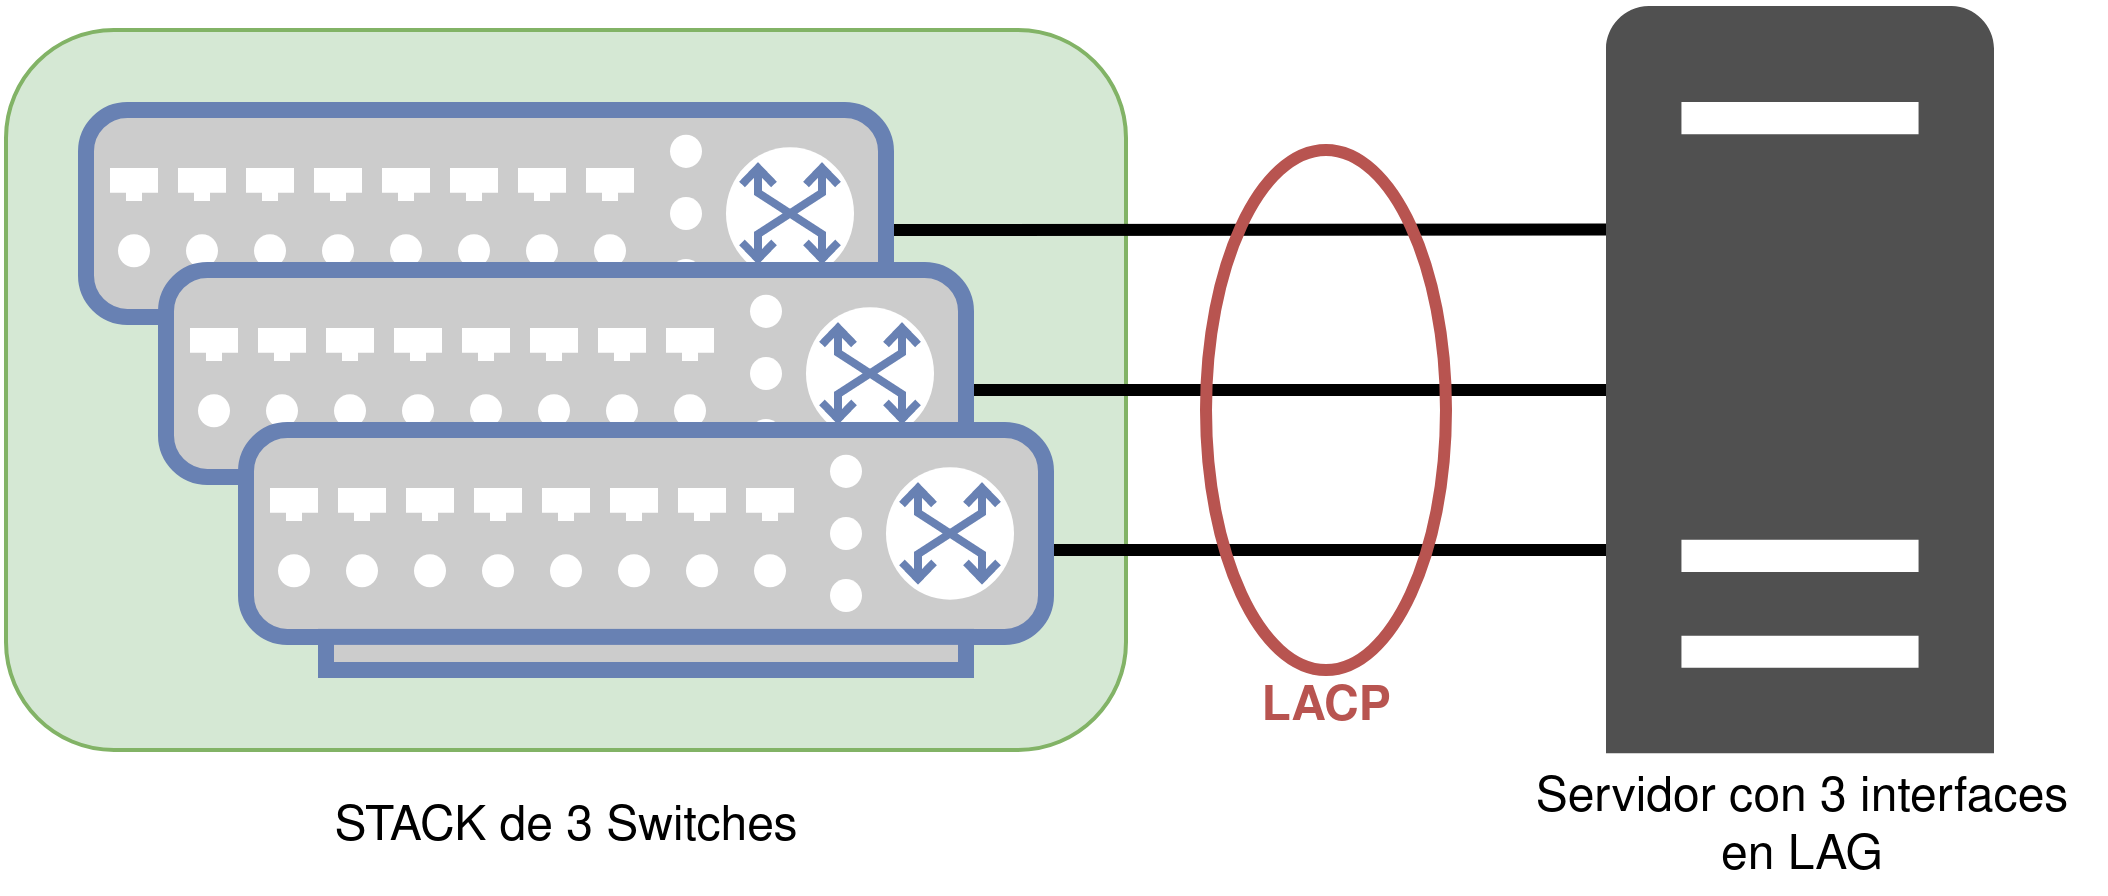
\includegraphics[width=0.6\linewidth]{LACP_stack_servidor.png}
    \vspace{-10pt}
\end{center}

Podemos observar cómo tenemos un stack de 3 switches, que como ya hemos visto previamente actúan como si se tratara de uno sólo. Por otro lado tenemos el servidor, que cuenta con 3 tarjetas ethernet que han sido configuradas a nivel de sistema operativo en modo LACP, y cada una de ellas se ha conectado a un switch distinto del stack.

\infobox{Con esta configuración, nos estamos asegurando que si un switch se estropea, la conectividad seguirá existiendo entre el servidor y el stack a través de los dos enlaces restantes.}

Es muy importante que nuestra infraestructura de red sea pensada para tener el menor número puntos de fallos posibles, y haciendo uso de stacks de switches y conexiones LACP podremos reducir esos puntos de fallo.

